% !TEX TS-program = pdflatexmk
\documentclass{./packages/optica-article}

\graphicspath{{images/}{practica2/images/}}

\journal{opticajournal}
\usepackage{csvsimple}
\usepackage{siunitx}
\usepackage{physics}
\usepackage{booktabs}
\usepackage{tikz}

\usepackage{caption}
\usepackage{subcaption}

% No floating captions
\usepackage{capt-of}
\usetikzlibrary{positioning}

\tikzset{>=stealth}

% cref instead of ref
\usepackage{cleveref}

%\usepackage[allfiguresdraft]{draftfigure}


\newcommand{\sinc}{\textrm{sinc}}
\newcommand\conv{\circledast}

% Set the article type
\articletype{Research Article}

% \usepackage{lineno}
% \linenumbers

\begin{document}

\title{Procesado óptico de la información}

\author{Adriana Mamani Lazarte\authormark{1} Alex G. Recuenco\authormark{1}, and Carlos España Castaño\authormark{1}}

\address{\authormark{1}Universidad Complutense de Madrid, Madrid, PC 28040, España}

\tableofcontents
\section{Introducción}
En la práctica realizada primeramente se aprendió a realizar montajes experimentales de sistemas ópticos, de tal manera que el mismo este alineado de manera correcta y el haz se encuentre colimado. 
Se estudia experimentalmente el efecto de Talbot que es la reproducción de campos periódicos durante la propagación en el espacio
libre en el régimen de Fresnel para ciertas distancias. 
Por otra parte, se construyó un sistema para la observación y medida del espectro de Fourier de un objeto 2D (en este caso una lámina fotográfica). 
Se analiza la difracción de la iluminación coherente de una imagen al mover la cámara con respecto a la imagen.


\subsection{Marco Práctico}
\subsubsection{Observación efecto de Talbot}

La primera parte de la práctica consistió en la observación de imágenes de la difracción de una onda plana coherente y monocromática en el régimen de Fresnel por un objeto periódico.
Se trabajó con un láser de 635nm, en el siguiente sistema en la cual la lente colimadora transforma la onda esférica divergente en una onda plana.

% Nota como para FORZARLO a estar aqui, no se utiliza figure, que es algo que flota
% Esto normalmente esse considera mala forma en un documento, ya que LaTeX es muy bueno a cuadrar todo
\begin{center}
	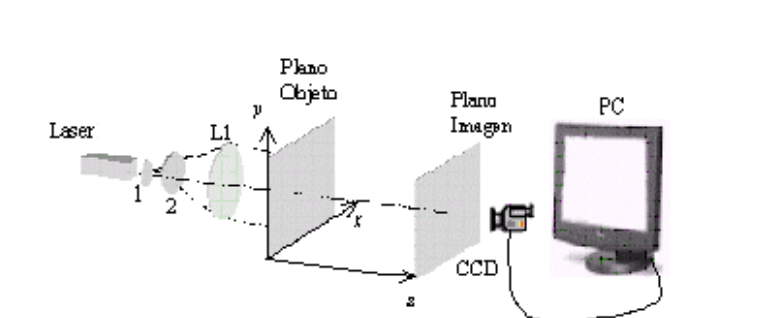
\includegraphics[scale=1]{sistematalbot.png}
	\captionof{figure}{Esquema del banco óptico, (1) filtro espacial, (2) atenuador, L1 lente colimadora, cámara CCD y PC para efectuar el registro.}
	\label{fig:talbot} % for use in \ref{table1} if you want to refer to the table number
\end{center}

\subsubsection{Espectro de Fourier}

Para obtener el módulo de la transformada de Fourier de una escena mediante sistemas ópticos se trabajó con un montaje que se componía por una lente delgada, cuyo plano de entrada está iluminado por un plano de luz, coherente y monocromático.

\begin{figure}[h]
	\centering
	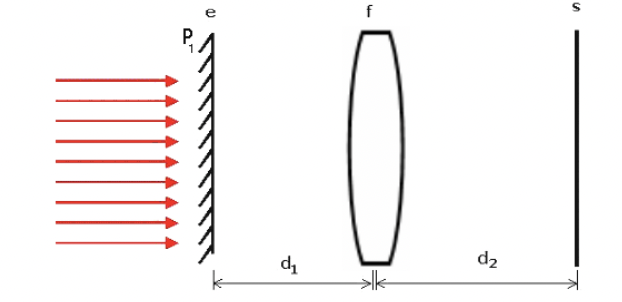
\includegraphics[scale=1]{sistemaespectrodefourier.png}
	\caption{Esquema del montaje experimental para la observación del espectro de Fourier de un objeto plano. }
	\label{fouriersistema}
\end{figure}

En el sistema armado se utilizaron lentes focales diferentes, un polarizador como atenuador y un diafragma para disminuir la influencia de luz parásita.

Se observaron los espectros de Fourier en distintos escenarios que expondremos en la parte de resultados de la práctica.

\subsubsection{Filtrado óptico}

Se realiza la práctica experimental de esta parte con el montaje de un sistema 4f introducido por Van der Lugt para el procesado óptico de información de 1963

\begin{figure}[h]
	\centering
	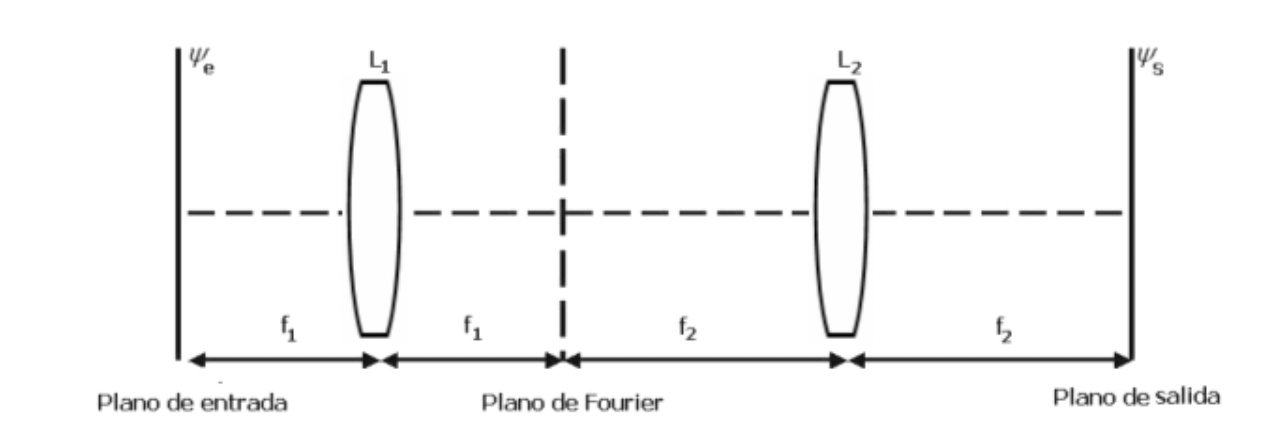
\includegraphics[scale=0.5]{/parte4-filtrado/Sistema3.png}
	\caption{Esquema para la realización de una operación de filtrado óptico.}
	\label{filtradoopticosistema}
\end{figure}

Compuesto por un objeto de una escena en el plano P1, que es el focal de la lente L1 se ilumina con una onda plana. 
En el otro plano focal de la lente L1 donde se obtendrá la transformada de Fourier del objeto.

\subsubsection{Formación de imagen con luz parcialmente coherente}

El grado de coherencia del haz afecta directamente a como un sistema óptico forma imagen, por lo tanto, controlaremos este parámetro. 
Por tanto, en el siguiente montaje con él trabajaremos.

\begin{figure}[h]
	\centering
	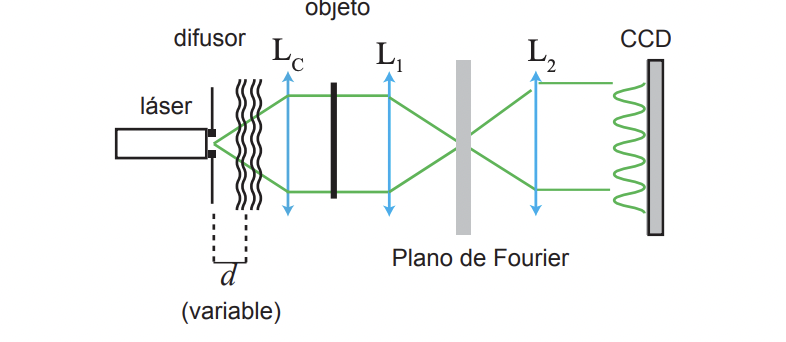
\includegraphics[scale=0.5]{/parte5-luz-coherente/sistema4.png}
	\caption{Esquema de el filtrado con difusor, }
	\label{fig:coherenciaespacial}
\end{figure}






\section{Observación del efecto Talbot}
Con una red periódica, con distancia de periodo desconocido $d$, se observan  distintas distancias desde el foco, y se apuntan cuatro distancias correspondientes a $z_m$, $z_{m-\flatfrac 1 4}$, $z_{m-\flatfrac 1 2}$, $z_{m-\flatfrac 3 4}$. 

Para ello, se observó la evolución del campo difractado al alejar la cámara CCD, y cuando el contraste es mínimo o máximo (Fig.~\ref{fig:alltalbot})  se apuntó las distancias correspondiente. Todas las distancias quedan recogidas en la tabla~\ref{ec:zt}.

Las distancias a las que se reproduce el campo periódico son ciertas fracciones de la denominada distancia de Talbot, 
que viene dada por la expresión

\begin{equation}
	z_T = \frac{2p^2}{\lambda}.
	\label{ec:zt}
\end{equation}


Donde $p$ es el periodo de la red. 
Registramos varias imágenes a distancias en la que se observaba una distribución de intensidad semejante a la del objeto original (franjas transparentes y opacas de igual tamaño), 
así como a distancias en las que se observaba una distribución de intensidad homogénea:

\begin{center}
	\begin{tabular}{ | m{2cm} | c | >{\centering}m{1.5cm} | } \hline
		Distribución de intensidad & Distancia & Distancia (fracción de $z_T$) \\ \hline
		Homogénea                  & $z_T/4$   & 18,5 cm                       \\
		Franjas claras y oscuras   & $z_T/2$   & 36,8 cm                       \\
		Homogénea                  & $3z_T/4$  & 55,8 cm                       \\
		Franjas claras y oscuras   & $z_T$     & 72,9 cm                       \\\hline
	\end{tabular}
	\captionof{table}{Distancias fraccionarias de la longitud de Talbot $z_T$,
     como se pueden observar en Fig.~\ref{fig:alltalbot}}\label{tab:talbot}
\end{center}

\begin{figure}[hptb]
	\begin{center}
		\begin{subfigure}[t]{0.45\textwidth}\centering
			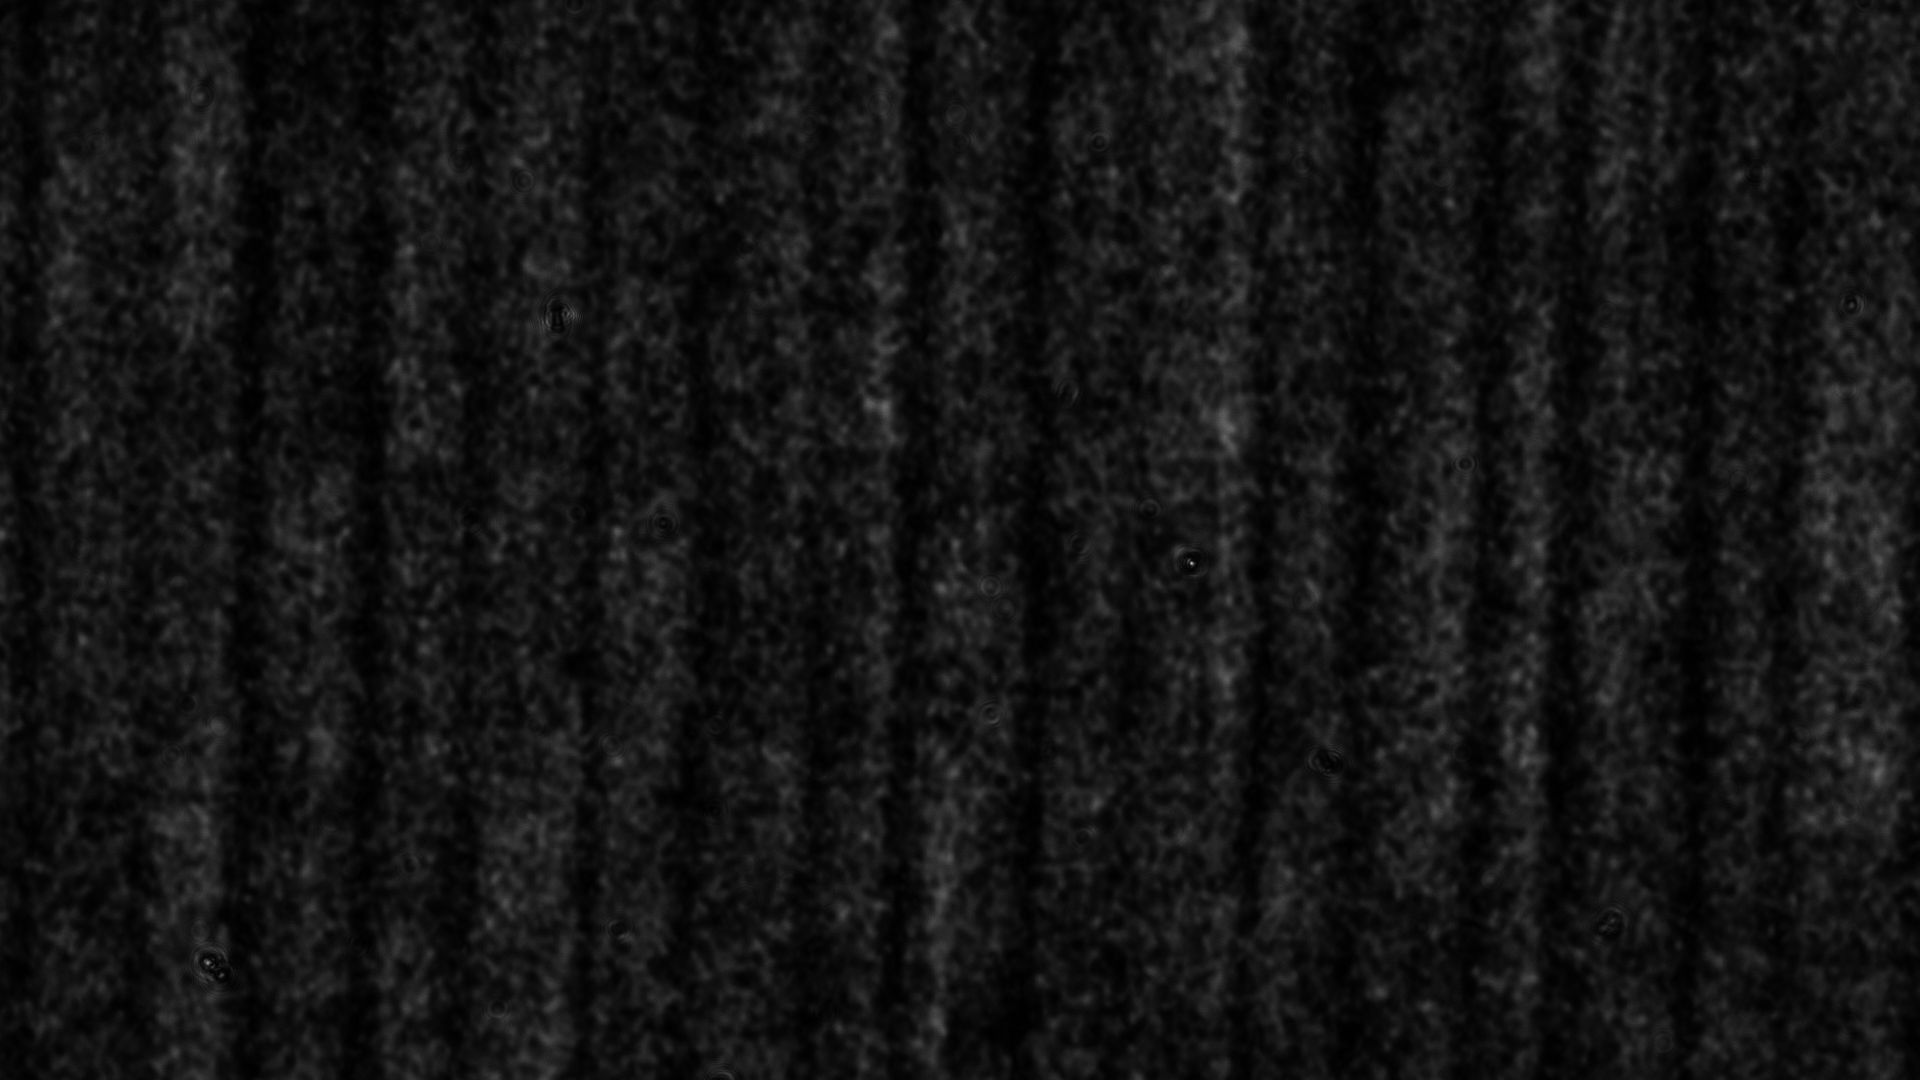
\includegraphics[width=\textwidth]{/parte2-talbot/4.9cm-talbot7.png}
			\caption{ Talbot a distancia 1 (18cm)}
			\label{fig:talbot1}
		\end{subfigure}
		\quad
		\begin{subfigure}[t]{0.45\textwidth}\centering
			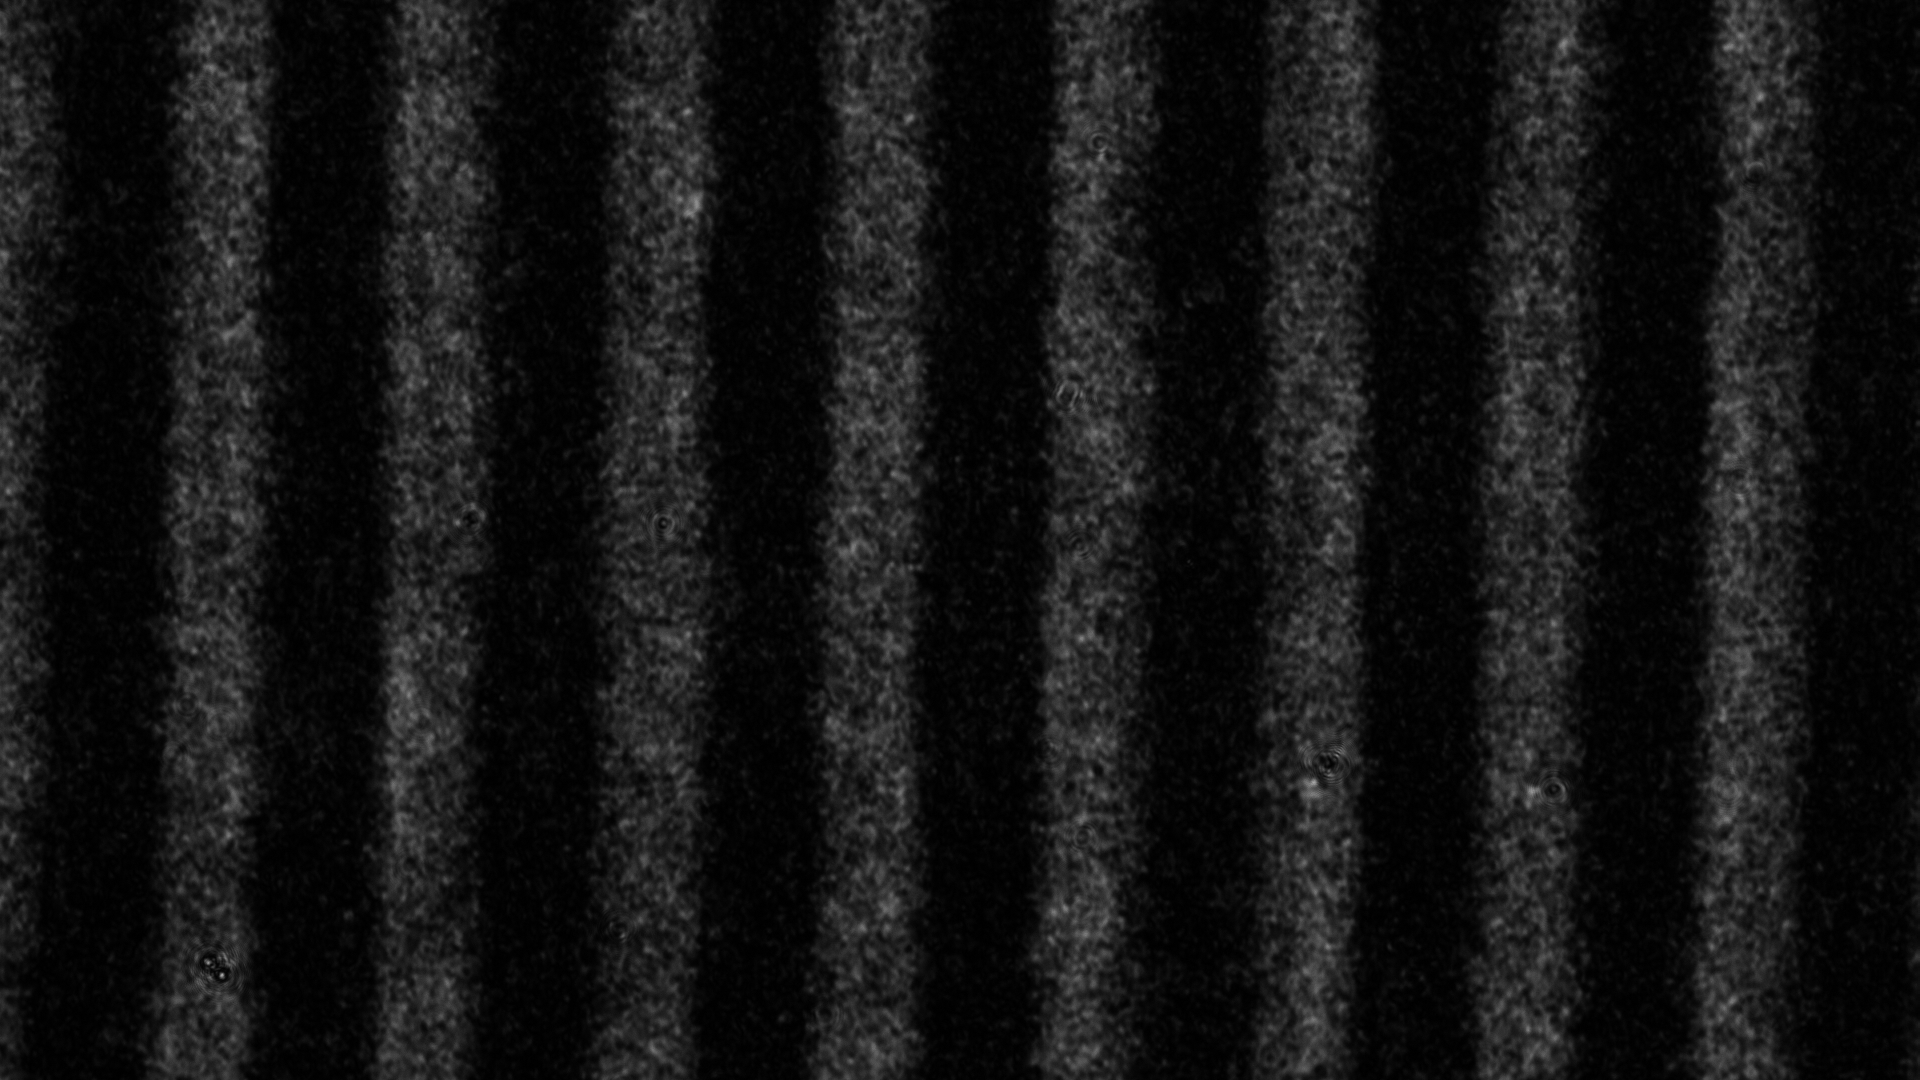
\includegraphics[width=\textwidth]{/parte2-talbot/23.9-talbot.png}
			\caption{Talbot a distancia 2 (36cm)}
			\label{fig:talbot2}
		\end{subfigure}
		\\
		\begin{subfigure}[t]{0.45\textwidth}\centering
			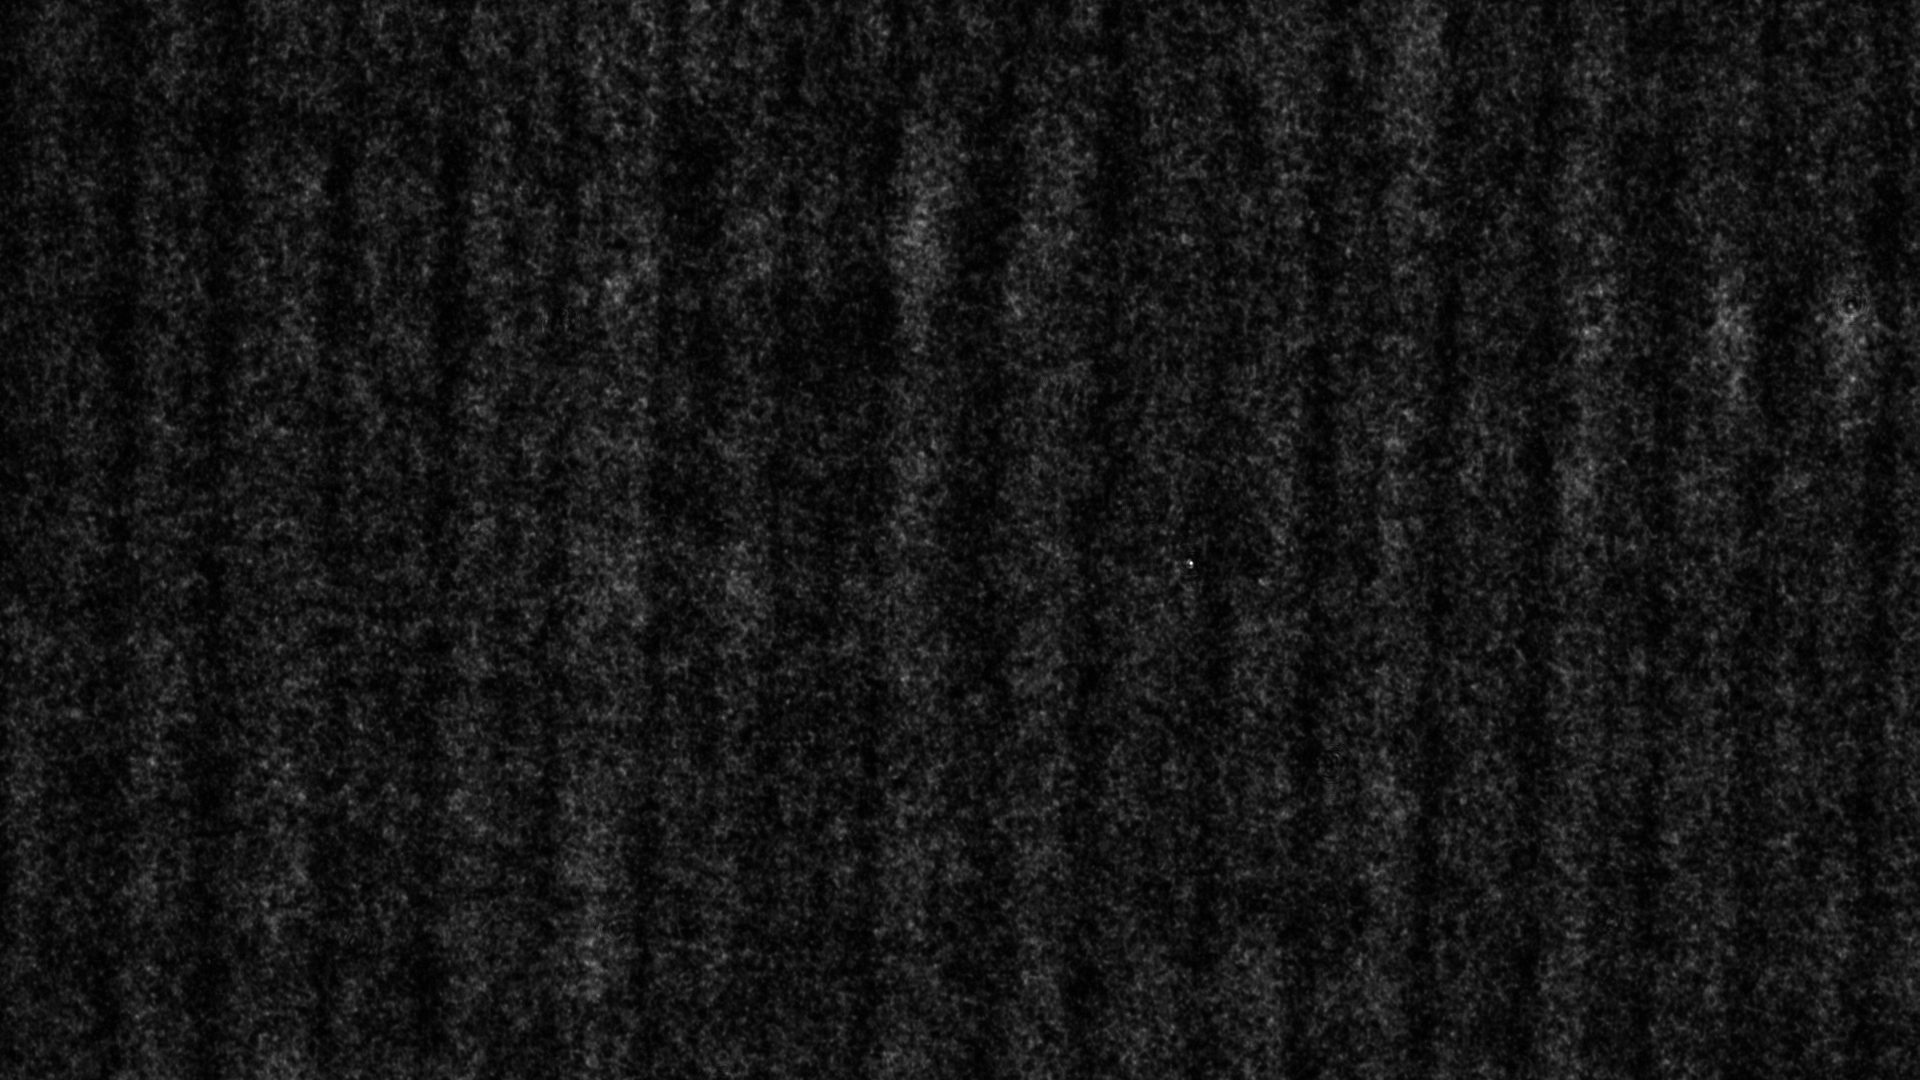
\includegraphics[width=\textwidth]{/parte2-talbot/42.2-talbot.png}
			\caption{ Talbot a distancia 3 (54cm)}
			\label{fig:talbot3}
		\end{subfigure}
		\quad
		\begin{subfigure}[t]{0.45\textwidth}\centering
			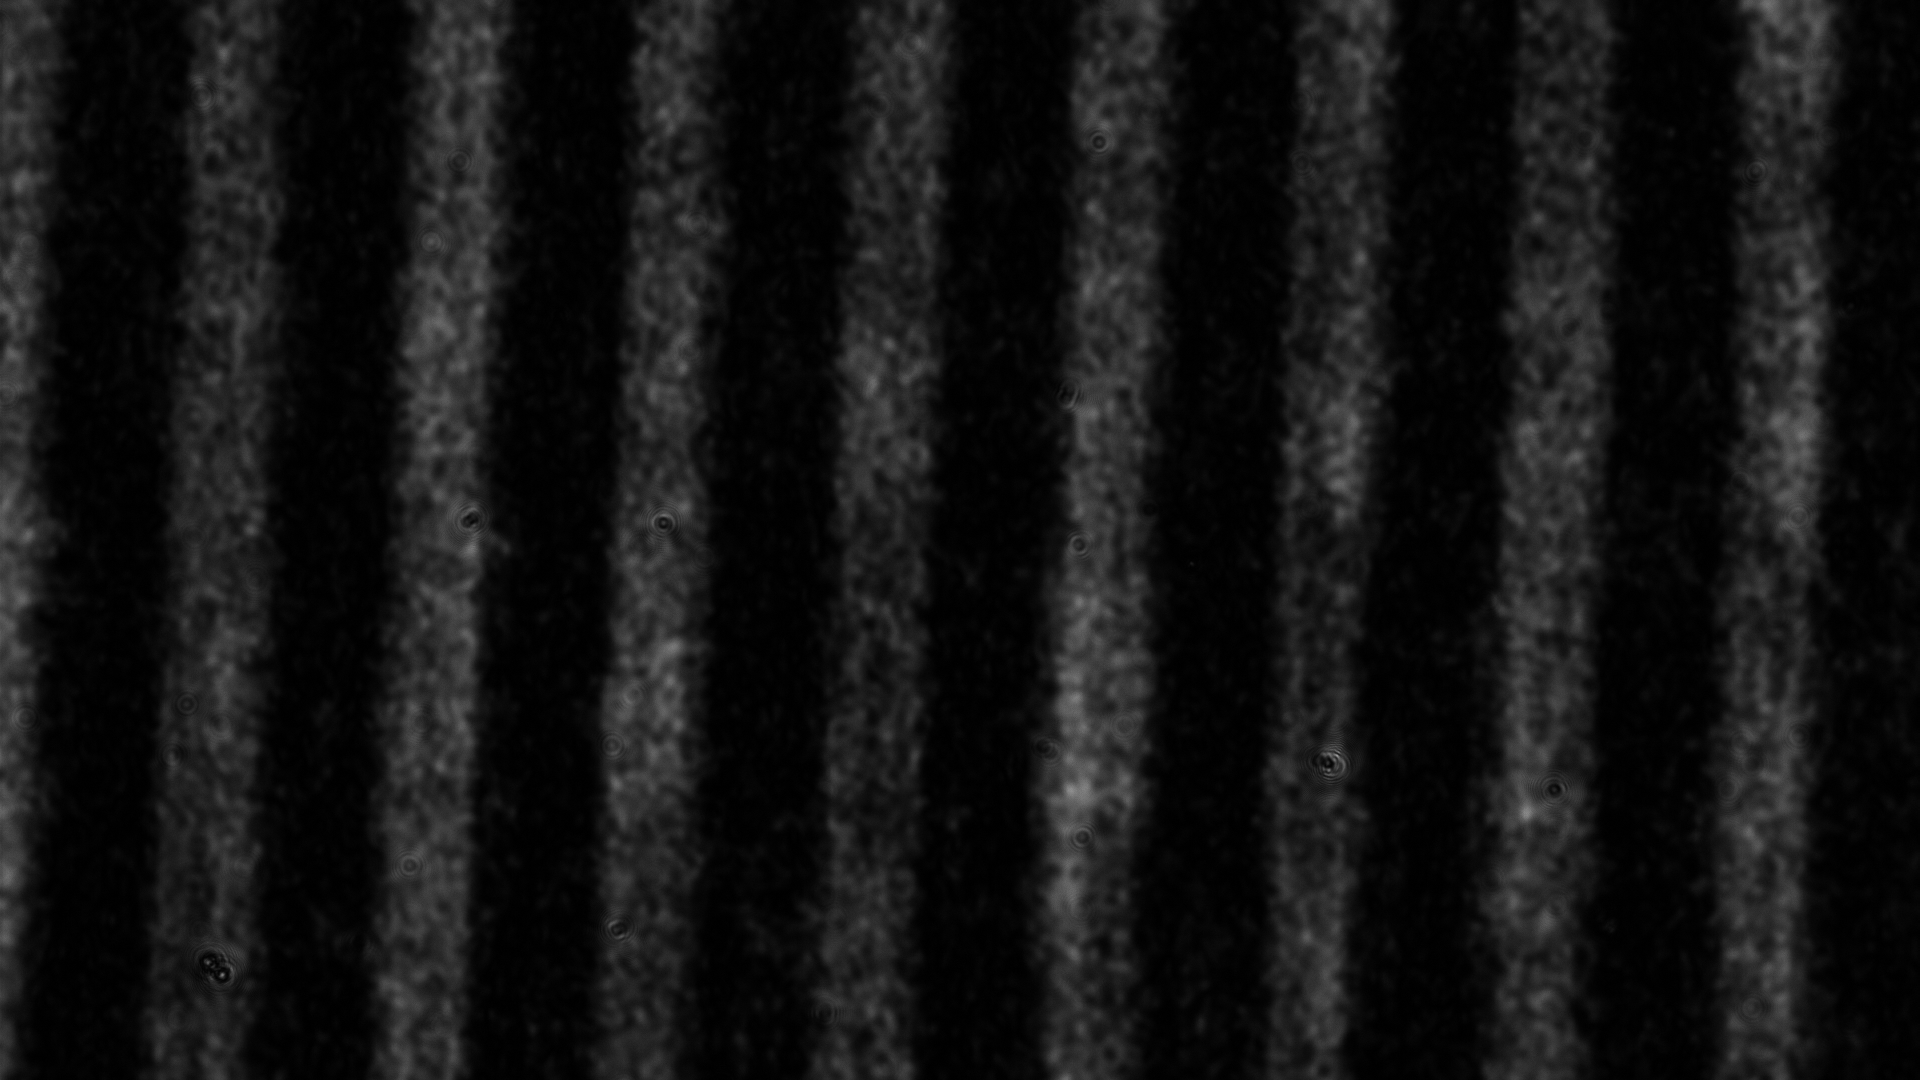
\includegraphics[width=\textwidth]{/parte2-talbot/54.8-2a-talbot.png}
			\caption{ Talbot a distancia 4 (73cm)}
			\label{fig:talbot4}
		\end{subfigure}

		\caption{Posiciones de contraste máximo (\ref{fig:talbot2}, \ref{fig:talbot4}) y mínimo (\ref{fig:talbot1}, \ref{fig:talbot3}).
			Se ve en estas fotos como entre \ref{fig:talbot2} y \ref{fig:talbot4} las posiciones tiene un shift de medio periodo.}
		\label{fig:alltalbot}
	\end{center}
\end{figure}

Periodo de la red:
En nuestro sistema, hemos encontrado que esta distancia vale $Z_T = 72,9 cm$. Conociendo la longitud de onda del láser, $\lambda = 635 nm$, se puede despejar el periodo de la red de la ecuación \ref{ec:zt}, obteniendo:
\begin{center}
	$p \approx 480 \mu m$
\end{center}


\subsection{Cuestiones}

Notese como referencia que el campo a una distancia $z$ de una red periodica es

\begin{equation}\label{eq:talbot}
	T(x, p z_t / q ) = \sum_{a=0}^{\flatfrac q 2 - 1} B(a, p, q) T (x - d/2 + 2ad/q, 0)
\end{equation}
Donde
\begin{align}
	\label{eq:talbot:t}
	B(a,p,q) & = \frac 2 q \sum_{b=0}^{\flatfrac q 2 - 1} e^{i 2 \pi \frac{2ba}{q} - i\pi \left(2 \flatfrac{p b^2}{q} + b\right)} \\
	T(x,0)   & =
	\sum_{n} a_n e^{\frac{i 2 \pi n x} {d}}                                                                                       \\
	T(x,z)   & =
	e^{ikz}
	\sum_{n} a_n e^{\frac{i 2 \pi n x} {d}} e^{- i n^2 \flatfrac{ \pi \lambda z } {d^2}}
\end{align}

\subsubsection{Representando una señal óptica periódica (longitud de onda $\lambda$, periodo $d$) como una serie de Fourier, demostrar analíticamente que en las distancias iguales a la mitad de la distancia de Talbot, $z=\flatfrac{z_{T}}{2}$, observamos el objeto original desplazado en la mitad del periodo $d$.}


A la mitad de la longitud de Talbot, aparece una auto-imagen, pero desfasada medio periodo.

Dada la ecuación.~\ref{eq:talbot:t}, si sustituimos $z_{m-1/2} = 2d^2/\lambda (m - 1/2)$
\nopagebreak
\begin{align*}
	T(x,z_{m - 1/2}) & =
	e^{ikz}
	\sum_{n} a_n e^{\frac{i 2 \pi n x} {d}} e^{- i n^2 \pi (2s - 1)} \\
	                 & =
	e^{ikz}
	\sum_{n} a_n e^{\frac{i 2 \pi n x} {d}} e^{ i n^2 \pi}           \\
	                 & =
	e^{ikz}
	\sum_{n} a_n (-1)^{n}e^{\frac{i 2 \pi n x} {d}}.                 \\
\end{align*}
Por lo tanto, en general, la intensidad es
\begin{equation}\label{eq:talbot:semi}
	I_{z_{m - 1/2}} = T \cdot T^{*}  =
	\sum_{n} \sum_{m} a_n a_{m}^{*} (-1)^{n + m}e^{\frac{i 2 \pi (n - m)  x} {d}}
\end{equation}
Realizando el calculo específico para una red periodica con transmitancia $t \propto 1 + \cos{2\pi x / d}$  con $a_0=1$, $a_{\pm 1}=1/2$, $a_n = 0$ si $\abs{n} > 1$
\nopagebreak
\begin{align*}
	T(x,z_{m-1/2}) & \propto
	e^{ikz}\left(
	1-1/2
	e^{\frac{i 2 \pi  x} {d}}-1/2
	e^{\frac{i 2 \pi  x} {d}}
	\right),                 \\
	I              & \propto
	\left(
	1-\cos (2 \pi  x / d)
	\right)^{2},
\end{align*}
En esta red periódica, es evidente que el efecto de mirar a $z=z_{m-1/2}$ estamos cambiando las franjas de mayor intensidad con aquellas de menor intensidad, cambiando los mínimos de intensidad con los máximos.
%  En general, no parece obvio a primera vista que esto siga siendo correcto para cualquier tipo de red.

\subsubsection{Usando la ecuación~\ref{eq:talbot} analizar la intensidad y la fase del campo difractado por un objeto periódico compuesto de líneas blancas (transparentes) y negras (opacas) alternadas de la misma anchura, a una distancia $z=\flatfrac{ZT}{4}$
}
De forma similar a eq.~\ref{eq:talbot:semi}, llegamos a
\begin{align}
	T(x,z) & =
	e^{ikz}
	\sum_{n} a_n e^{\frac{i 2 \pi n x} {d}}e^{i n^{2} \pi / 2}.
\end{align}

Evaluandolo la intensidad en una red con transmitancia $t \propto 1 + \frac{1}{2}\cos{2\pi x / d}$  con $a_0=1$, $a_{\pm 1}=1/4$, $a_n = 0$ si $\abs{n} > 1$
obtenemos
\nopagebreak
\begin{align*}
	T(x,z_{m-1/4}) & \propto
	e^{ikz}\left(
	1
	+i/4 e^{\frac{i 2 \pi  x} {d}}
	+i/4 e^{\frac{i 2 \pi  x} {d}}
	\right) = e^{ikz}
	\left(
	1
	+i/2 \cos(i 2 \pi  x /d)
	\right)
	,                                         \\
	I              & =  T \cdot T^{*} \propto
	\left(
	1
	+i/2 \cos(i 2 \pi  x /d)
	\right)
	\left(
	1
	-i/2 \cos(i 2 \pi  x /d)
	\right)                                   \\
	               & \propto
	1 - 1/4 \cos^{2}(i 2 \pi  x /d).
\end{align*}

A $z = z_{m - 1/4}$ por lo tanto se obtiene un contraste reducido en las franjas comparado con el original, y unos máximos más delgados.



\subsubsection{Justifique el procedimiento seguido para determinar la distancia de Talbot y el periodo de la red y exponga los resultados.}

Cuando una onda plana incide sobre una red de difracción periódica, la imagen de la red se repite a distancias regulares lejos del plano de la misma. Para encontrar la distancia de Talbot, realizamos el siguiente procedimiento:

\begin{enumerate}
	\item Usamos un sistema 4-f, y encontramos el plano de foco con un sistema no periódico, así no aseguramos que el punto de foque que encontramos es real, y no una imágen de Talbot
	\item Después, encontramos mientras nos trasladamos hacia atrás los puntos de $z_{1}/4$, $z_{1}/2$, $3 z_{1}/4$, $z_{1}$. Que podemos distinguir por medio de qué imágenes tienen contraste máximo/mínimo mientras nos desplazamos. como se ven en las Figuras~\ref{fig:alltalbot}.
	\item Así nos aseguramos que al tomar las cuatro distancias llegamos a la distancia primera de Talbot, no a un múltiplo o a una distancia de medio punto.
\end{enumerate}

\subsubsection{¿Las imágenes observadas siempre son periódicas? ¿La respuesta está de acuerdo con la teoría?}

A distancias mayores a las de Talbot mencionadas aparecen otras auto-imágenes que no conservan su periodicidad axial.


\section{Observación del espectro de Fourier}
Se toma los espectros de Fourier de las imágenes en cuestión presentadas a continuación en la figura ~\ref{fig:fourier:all}, donde se analizan sus características.

Podemos determinar el periodo de la red a partir de la distancia medida en el espectro de Fourier entre el máximo central y el máximo del primer armónico. Para ello, tenemos en cuenta que la expresión que relaciona el campo a la entrada de la lente con el campo en el plano focal (ec. ~\ref{ec:tf-plano-focal})

\begin{equation}
    E(u,\,f') \propto \textrm{TF}\{E_{in}\}\left(\frac{k}{f'}u\right)
    \label{ec:tf-plano-focal}
\end{equation}

La variable de la transformada de Fourier del objeto está escaladas con un factor $\frac{k}{f'}$, donde $k=\frac{2\pi}{\lambda}$ y f' es la distancia focal de la lente. La transformada de Fourier de la onda cuadrada, $\textrm{square}(x)$, es, en la dirección $y$ una delta, $\delta y$, y en la dirección $x$ una suma discretizada de deltas (multiplicadas por un factor):

\begin{equation}
    \textrm{TF}\qty\{square(x)\}\qty(\frac{k}{f'}u) = \frac{A}{2} + \frac{A}{\pi}  \delta\left(\frac{k}{f'} u - \nu_0\right) + \frac{A}{3\pi} \delta\left(\frac{k}{f'}u - 3\nu_0\right) + \ldots
\end{equation}

Donde $\nu_0 = \frac{1}{p}$ es la frecuencia de la onda cuadrada, siendo $p$ el periodo, y $A$ es la amplitud. Vemos en esta ecuación que el pico del primer armónico estaría desplazado $\frac{f'}{k} \nu_0$ respecto del pico central, en unidades de u. La distancia entre este pico central y el primer armónico, llamémosla d, es por tanto:

\begin{equation}
    d = \frac{\nu_0 f'}{k} = \frac{f'\lambda}{2\pi \cdot p}
    \label{ec:d-p}
\end{equation}

Podemos medir la distancia $d$ utilizando el programa ImageJ. Utilizando la imagen captada con la lente de $f' = 20$, la distancia nos da un resultado de $120 px$. Con un tamaño del píxel de $2,2 \unit{\micro\meter}$, la distancia en micras es es $d = 264 \unit{\micro\meter}$. Con una longitud de onda de $\lambda = 635 \unit{\nano\meter}$, usamos~\ref{ec:d-p} obteniendo:
% Usamos a~\ref{} porque ~ es un espacio irrompible.  Si utilizas a ~\ref{}. Tienes dos espacios, uno irrompible, y otro normal.

\begin{center}
    $p = 130 \unit{\micro\meter}$
\end{center}

\begin{figure}[hptb]
	\begin{center}
		\begin{subfigure}[t]{0.45\textwidth}\centering
			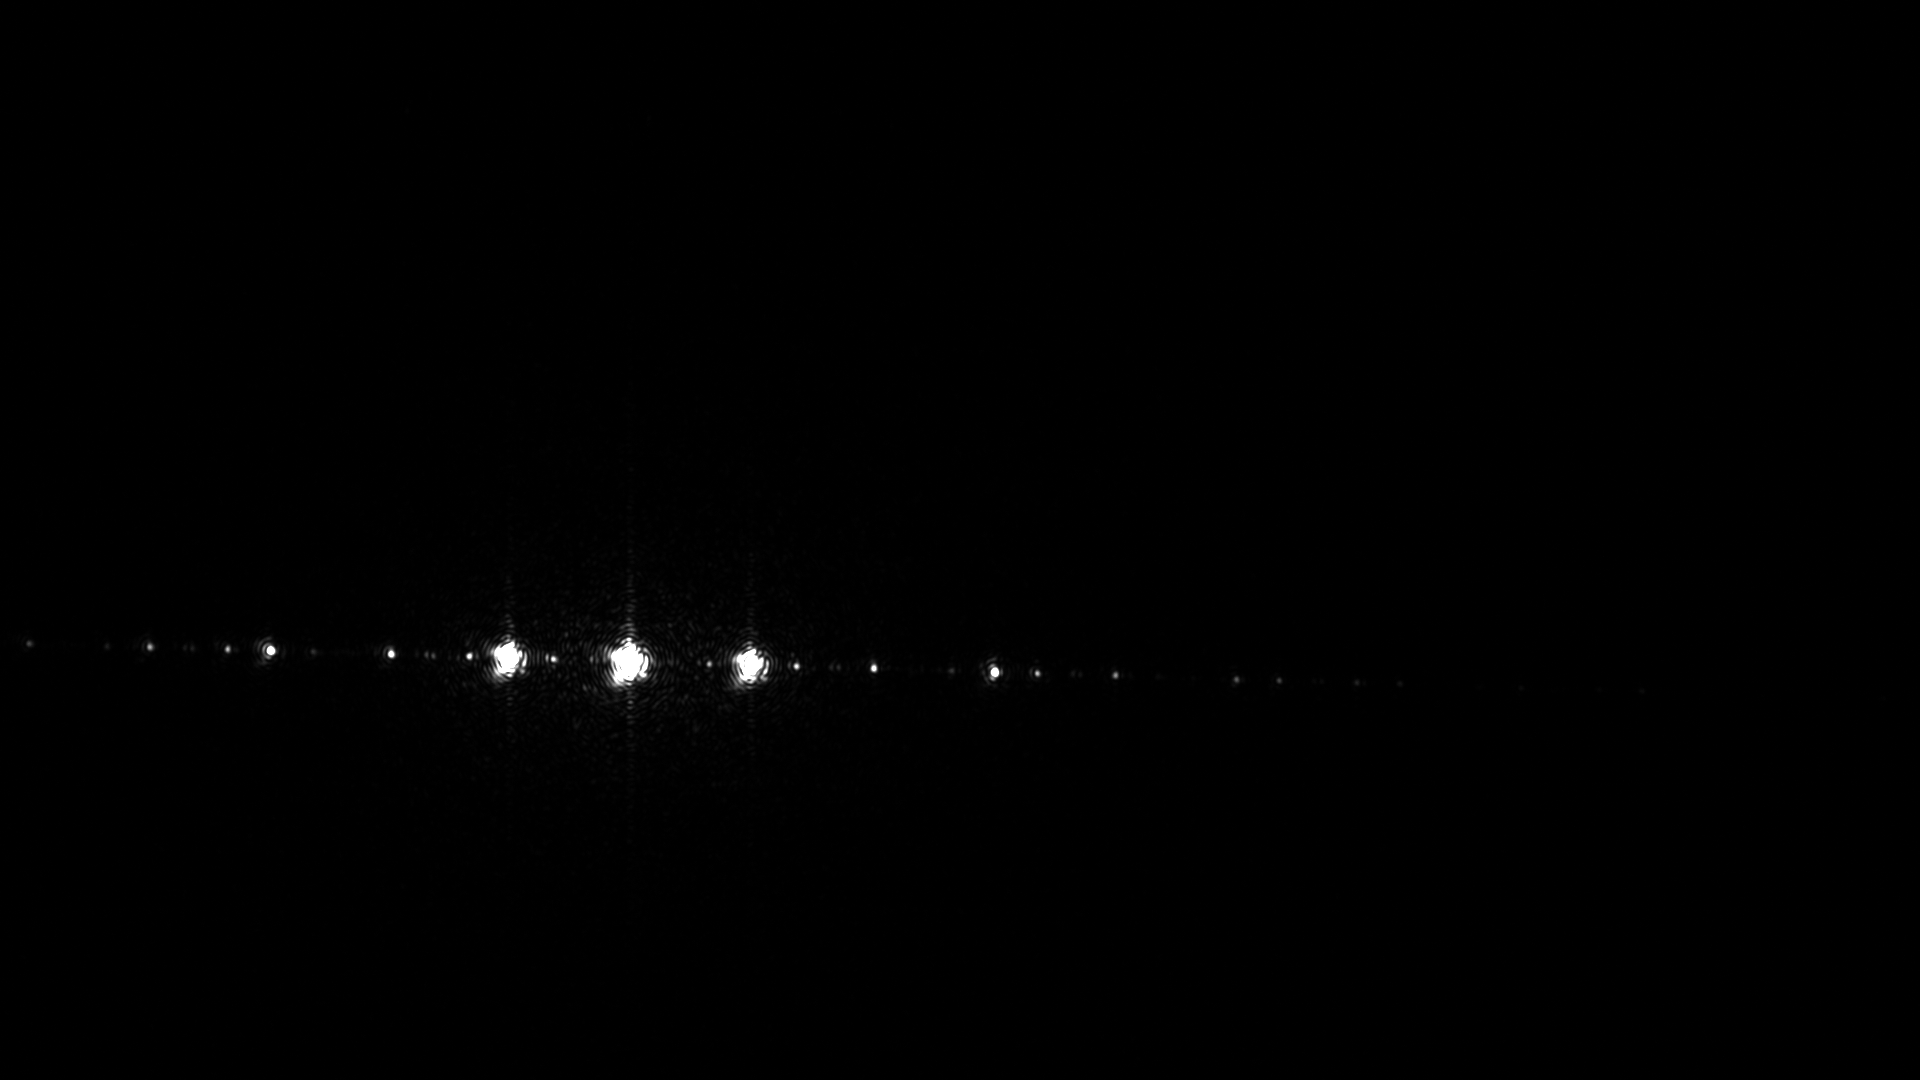
\includegraphics[width=\textwidth]{/parte3-fourier/fourier_transform_-20-lense-20-camera.png}
			\caption{Espectro de Fourier de líneas verticales  con una lente de focal de 20cm. Nótese como teóricamente la transformada de Fourier debería ser discreta, incluyendo los órdenes impares. El error experimental (líneas no vertical, alineamiento, aberración, etc), vemos pequeños valores para los órdenes pares}
			\label{fig:fourier1}
		\end{subfigure}
		\quad
		\begin{subfigure}[t]{0.45\textwidth}\centering
			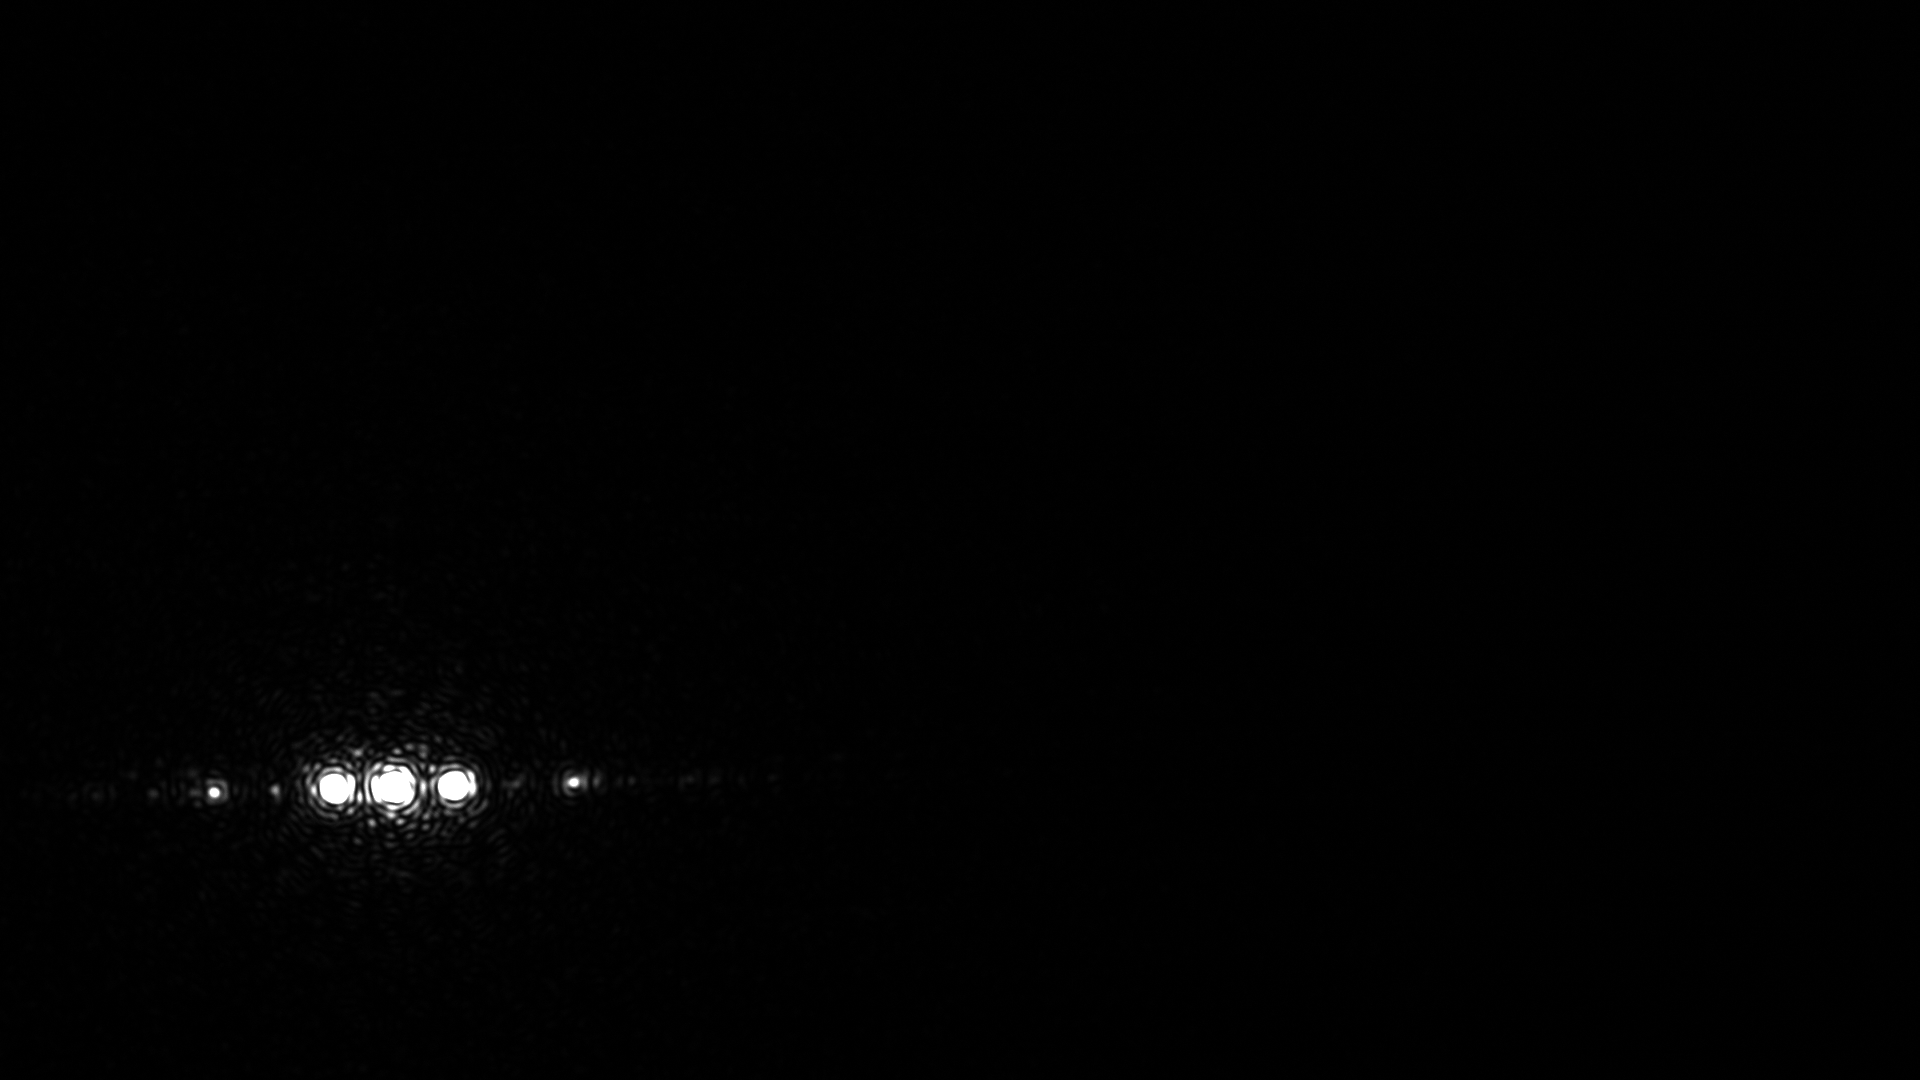
\includegraphics[width=\textwidth]{/parte3-fourier/fourier-periodic-grating-10cm-focal.png}
			\caption{Espectro de Fourier de líneas con una lente de 10cm de focal. Nótese el efecto que tiene en crear una imagen igual que \ref{fig:fourier1} pero mas pequeña}
			\label{fourier4}
		\end{subfigure}

		\begin{subfigure}[t]{0.45\textwidth}\centering
			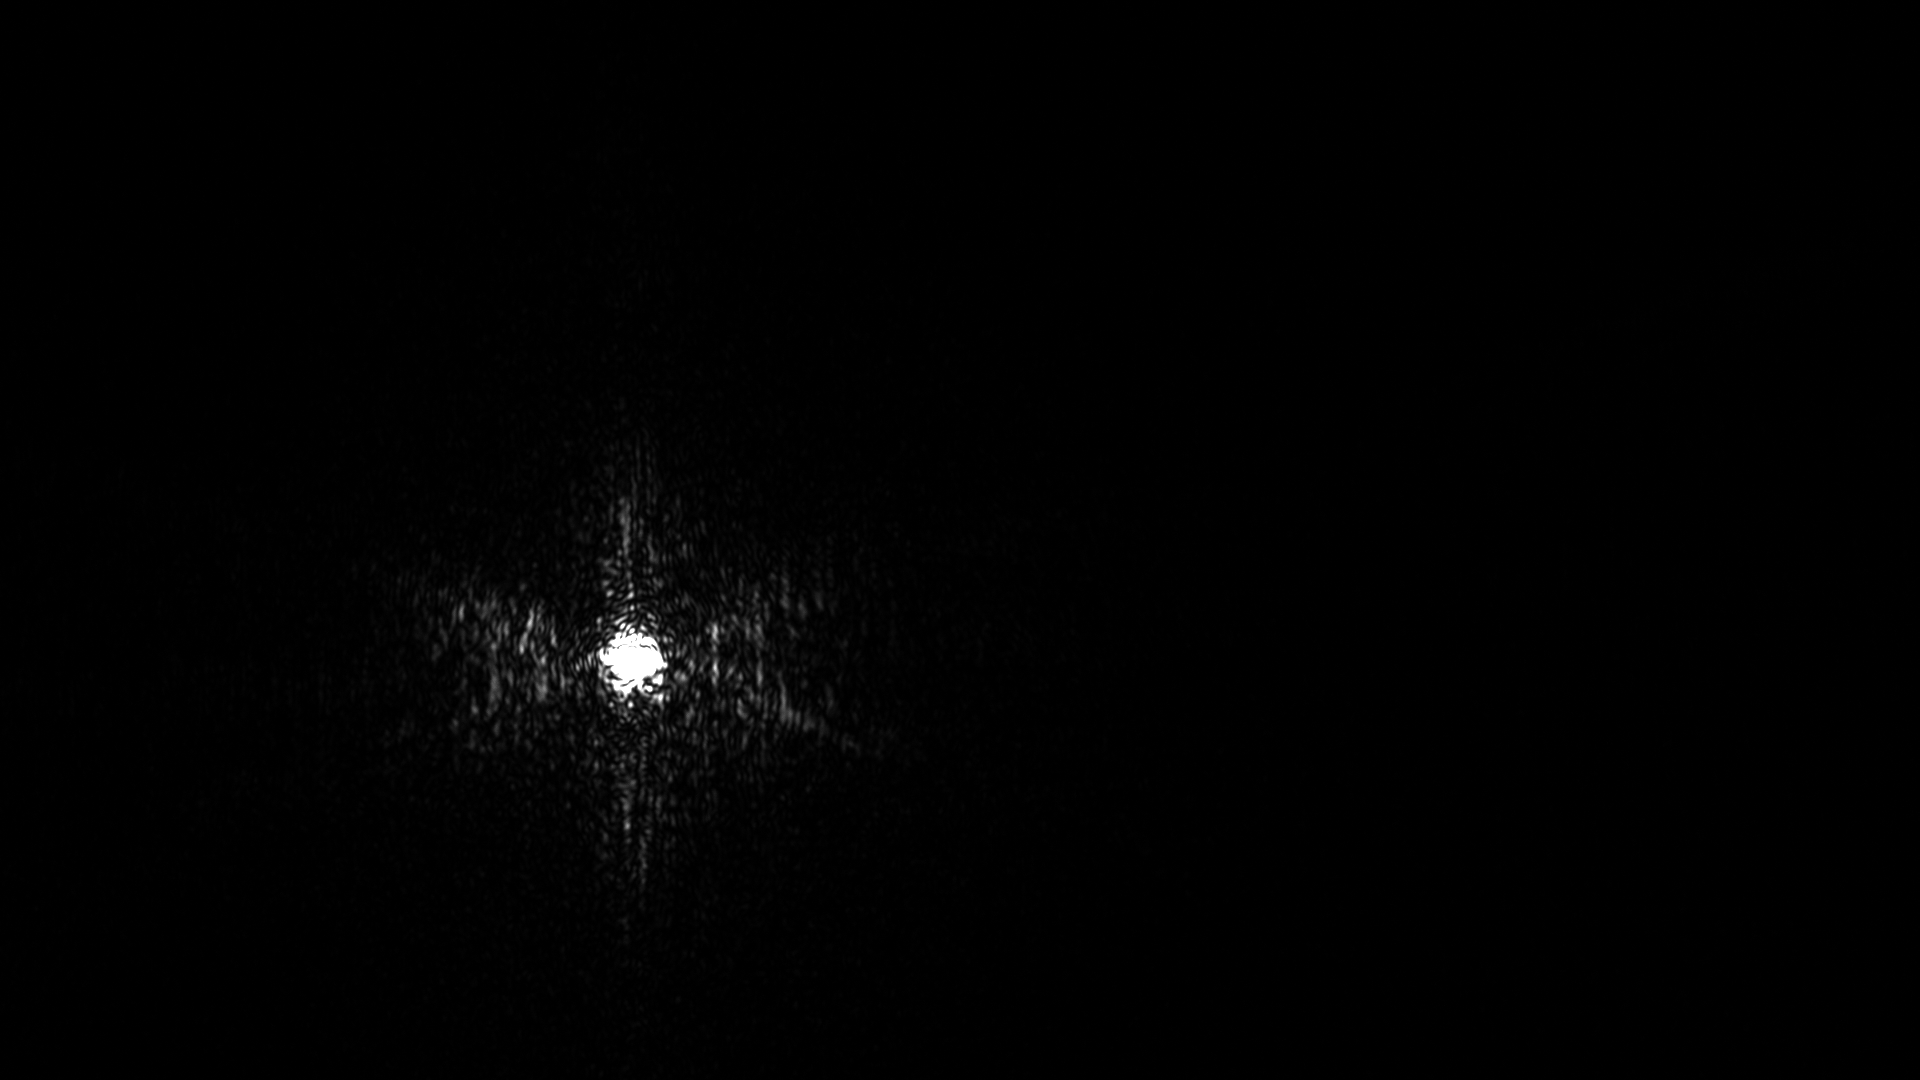
\includegraphics[width=\textwidth]{/parte3-fourier/fourier-letras.png}
			\caption{Espectro de Fourier de las letras. Nótese que al tener mejor resolución que el coche (\ref{fig:fourier2}) no se ve el tamaño de píxel reflejado}
			\label{fourier3}
		\end{subfigure}
		\quad
		\begin{subfigure}[t]{0.45\textwidth}\centering
			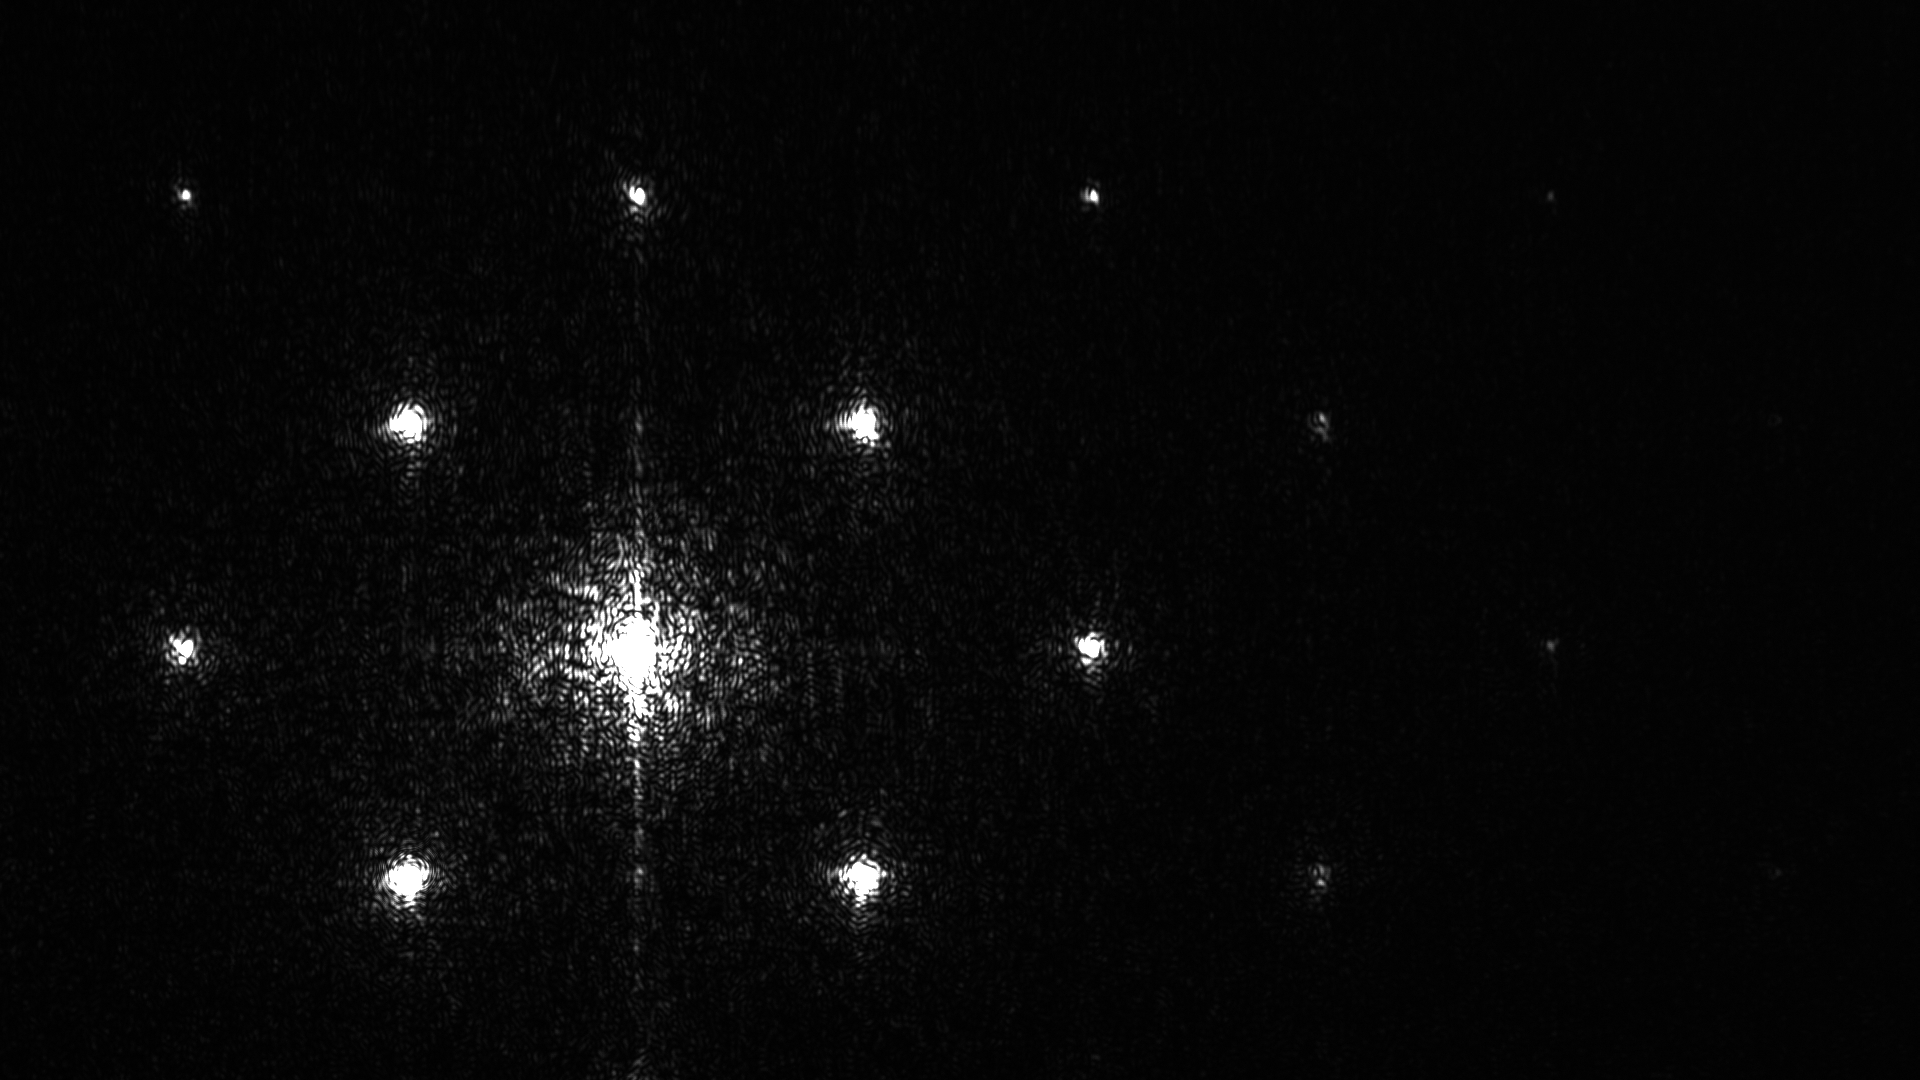
\includegraphics[width=\textwidth]{/parte3-fourier/fourier-car-multiplied-pixels.png}
			\caption{Espectro de Fourier de una imagen de un automóvil. Nótese que la imagen tiene un tamaño de pixel suficientemente grande para que los píxeles en sí forman un \emph{square grating}. Por lo tanto, lo que estamos viendo es la convolución de un \emph{square grating} con la foto del coche, lo que crea la misma imagen de Fourier del coche trasladada a cada orden de la rendija cuadrada.}
			\label{fig:fourier2}
		\end{subfigure}
		\caption{Observaciones en campo de Fourier de distintos elementos}\label{fig:fourier:all}
	\end{center}
\end{figure}

\subsection{Cuestiones}
\subsubsection{ ¿Qué valores $d_1$ y $d_2$ son adecuados para la observación del espectro de Fourier?}
La distancia de $d_{1}$ no importa cuando la onda incidente es plana. El desplazamiento solamente introduce un término de fase que no se modifica la intensidad observada. La distancia $d_{2}$ tiene que ser la focal de la lente, para que en el plano de observación obtengamos una imagen escalada de la transformada de Fourier.

\subsubsection{¿El espectro de la red está de acuerdo con la teoría (véanse los resultados del problema 1.6.)?}
Véase la descripción de~\ref{fig:fourier:all}.
Como se explica en esa descripción, sí, se ajusta con la teoría, excepto que ciertos errores permiten que los órdenes pares tengan valores no nulos, en vez de ser exactamente cero.

\subsubsection{ Justifique el procedimiento seguido para determinar el periodo de la red y exponga los resultados.}
El espectro de onda plana es un espectro continuo de ondas planas uniformes y hay un componente de onda plana en el espectro para cada punto tangente en el frente de fase de campo lejano. La amplitud de ese componente de onda plana sería la amplitud del campo óptico en ese punto tangente. Nuevamente, esto es cierto solo en el campo lejano, es por lo cual observamos las imágenes resultantes de la transformada de Fourier de acuerdo a la naturaleza de la imagen en cuestión. Y es, por tanto, que el factor de escala de la TF depende de la distancia.

\subsubsection{¿Es posible registrar el espectro de Fourier colocando un objeto detrás de la lente?}

No porque el campo del objeto necesita transmitirse a través de la lente para obtener el espectro de Fourier en el plano focal, y para ello no importa dónde se sitúe el objeto, pero siempre delante de la lente. Si colocamos el objeto detrás de la lente, los patrones de intensidad que obtengamos no vendrán de rayos transmitidos a través de esta. La única posibilidad sería registrar la intensidad en campo lejano, pero se perdería mucha visibilidad.



\section{Filtrado óptico}
Se obtienen los siguientes resultados, descritos en la Fig.~\ref{fig:filtrado:all}:

\begin{figure}[hptb]
	\begin{center}
		\begin{subfigure}[t]{0.45\textwidth}\centering
			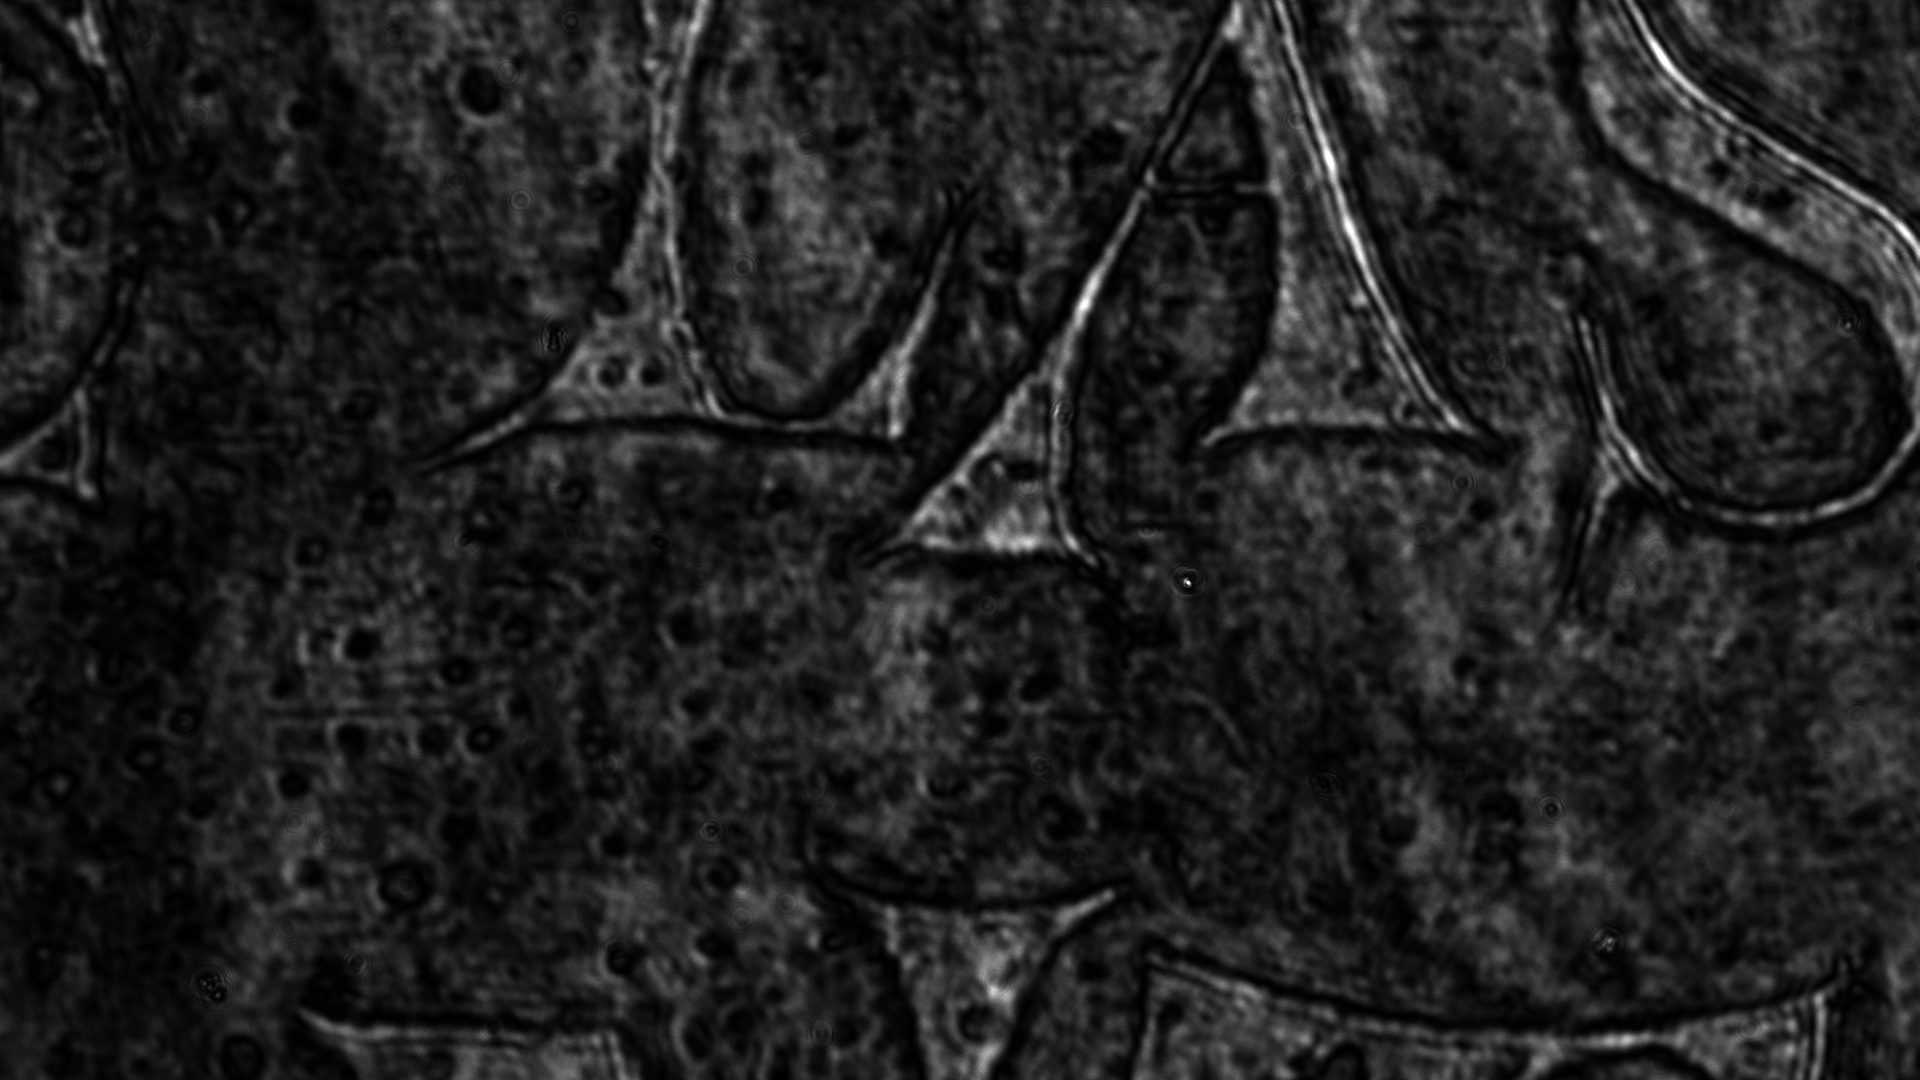
\includegraphics[width=\textwidth]{parte4-filtrado/4f-pic-2ocm-diafragm-10cm-camera-letters-diafragma_y_punto-pasabanda.png}
			\caption{Filtro con diafragma pasa banda, se puede ver en la imagen como esto elimina los bordes}
			\label{fig:filtrado1}
		\end{subfigure}
		\quad
		\begin{subfigure}[t]{0.45\textwidth}\centering
			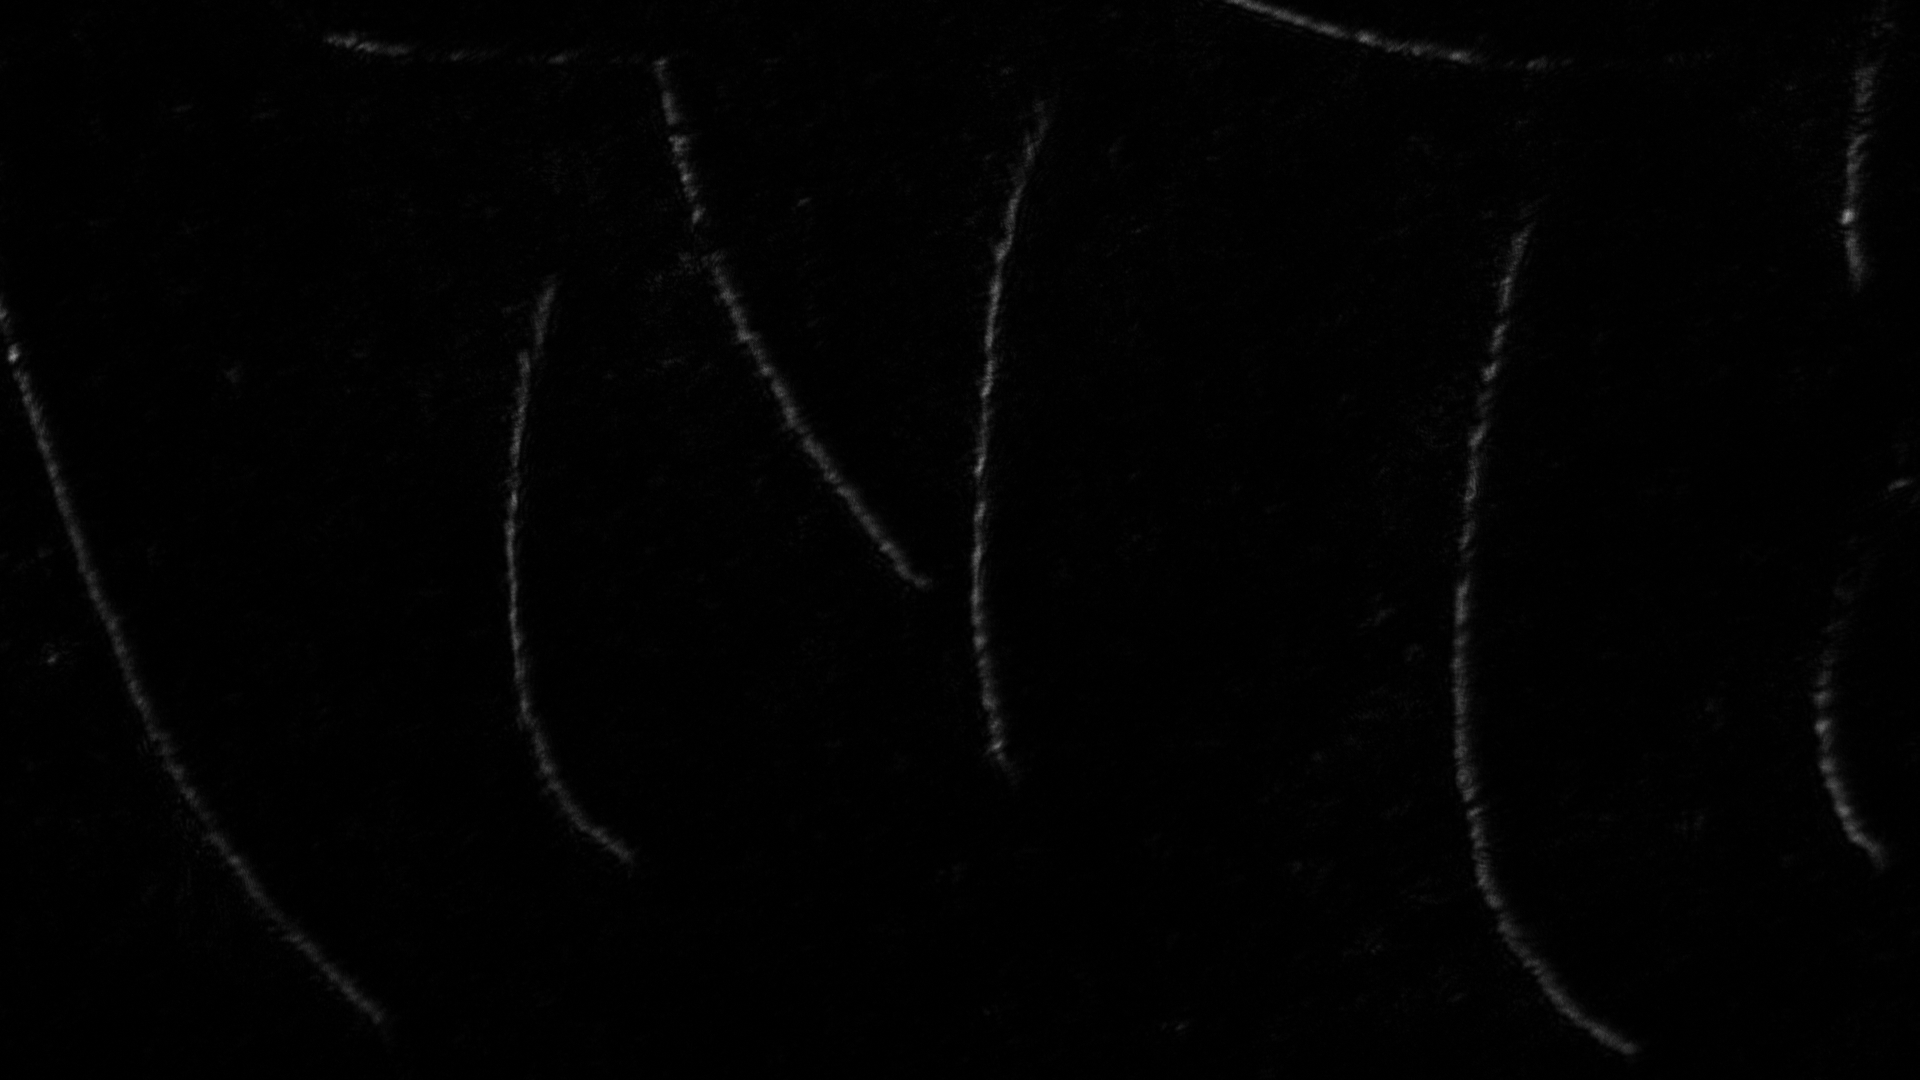
\includegraphics[width=\textwidth]{parte4-filtrado/4f-pic-2ocm-diafragm-10cm-camera-letters-high-frequency-almost-x.png}
			\caption{Filtrado pasa alta en la dirección horizontal, se realiza con un diafragma que corta el centro del foco en la dirección horizontal}
			\label{fig:filtrado2}
		\end{subfigure}
		\begin{subfigure}[t]{0.45\textwidth}\centering
			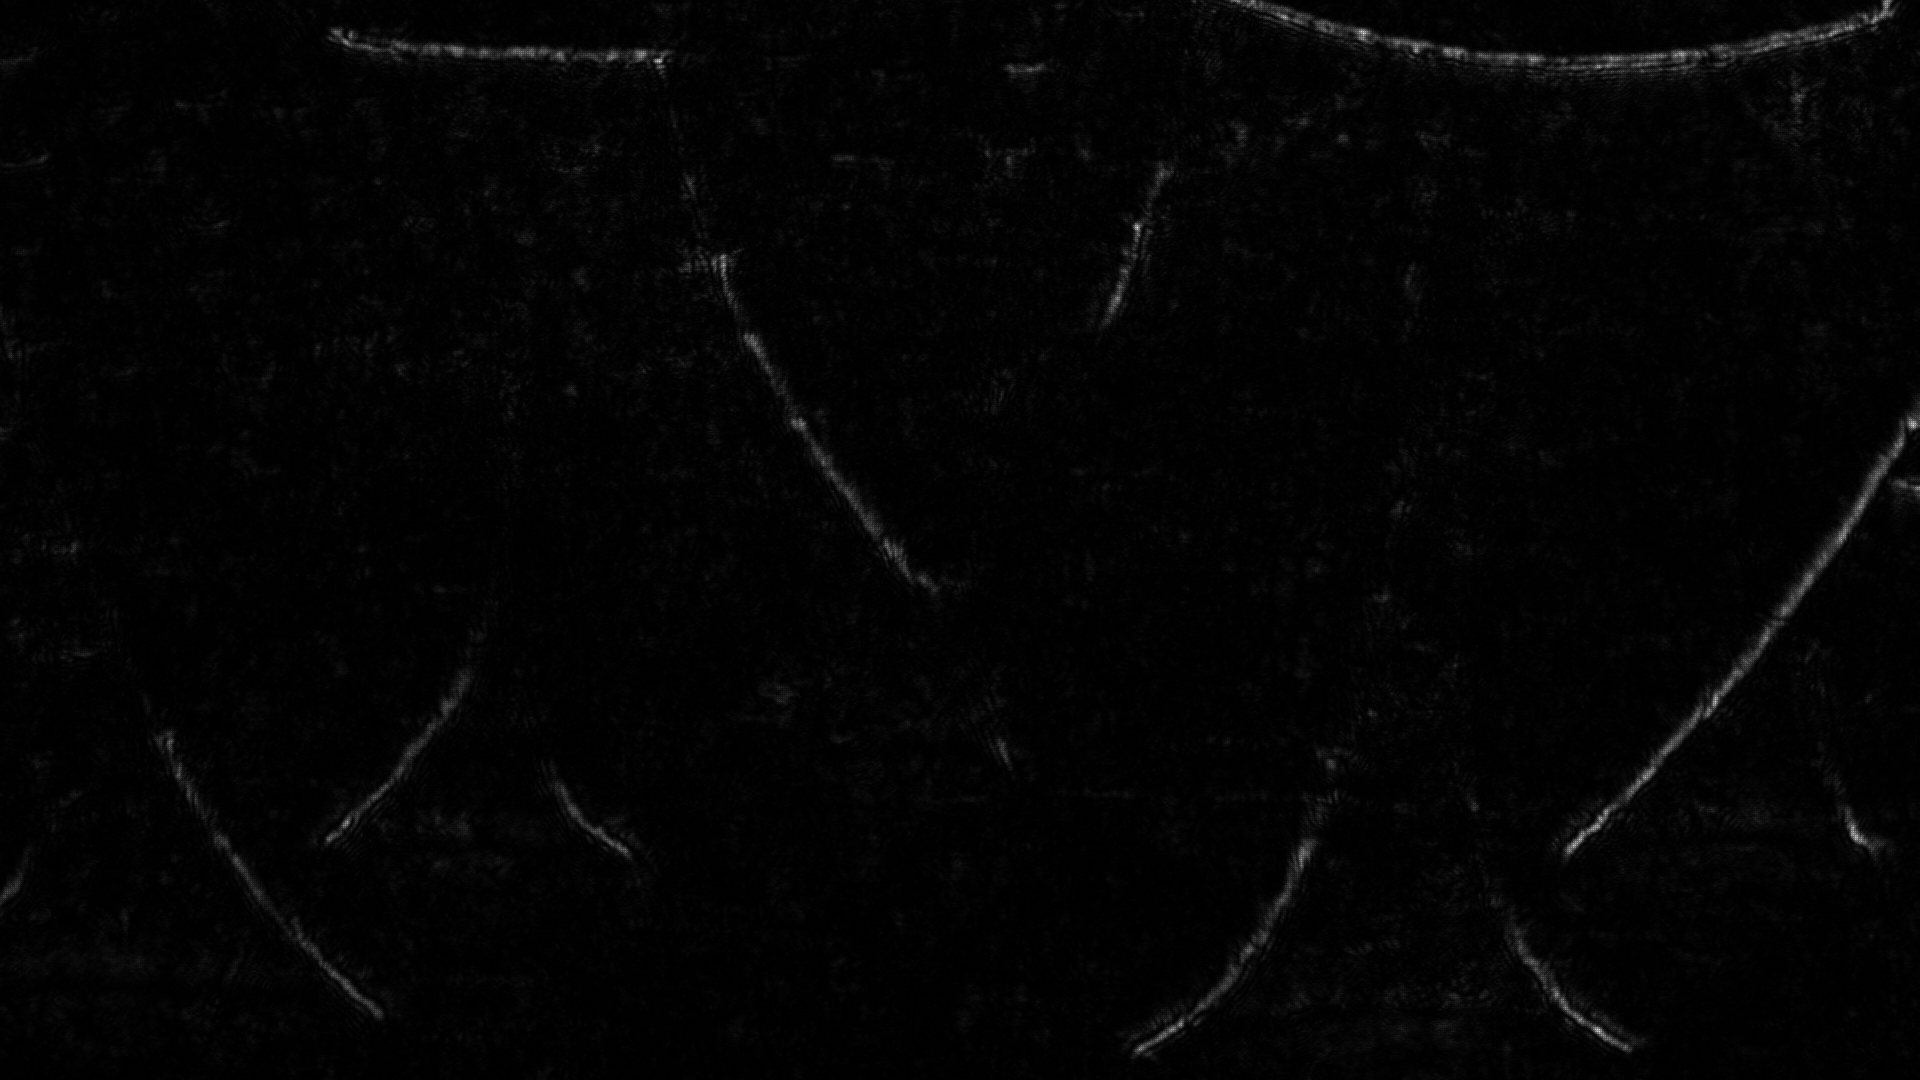
\includegraphics[width=\textwidth]{parte4-filtrado/4f-pic-2ocm-diafragm-10cm-camera-letters-high-frequency-dot-down.png}
			\caption{Filtrando de forma similar a \ref{fig:filtrado2}, pero en la dirección vertical}
			\label{fig:filtrado3}
		\end{subfigure}
		\quad
		\begin{subfigure}[t]{0.45\textwidth}\centering
			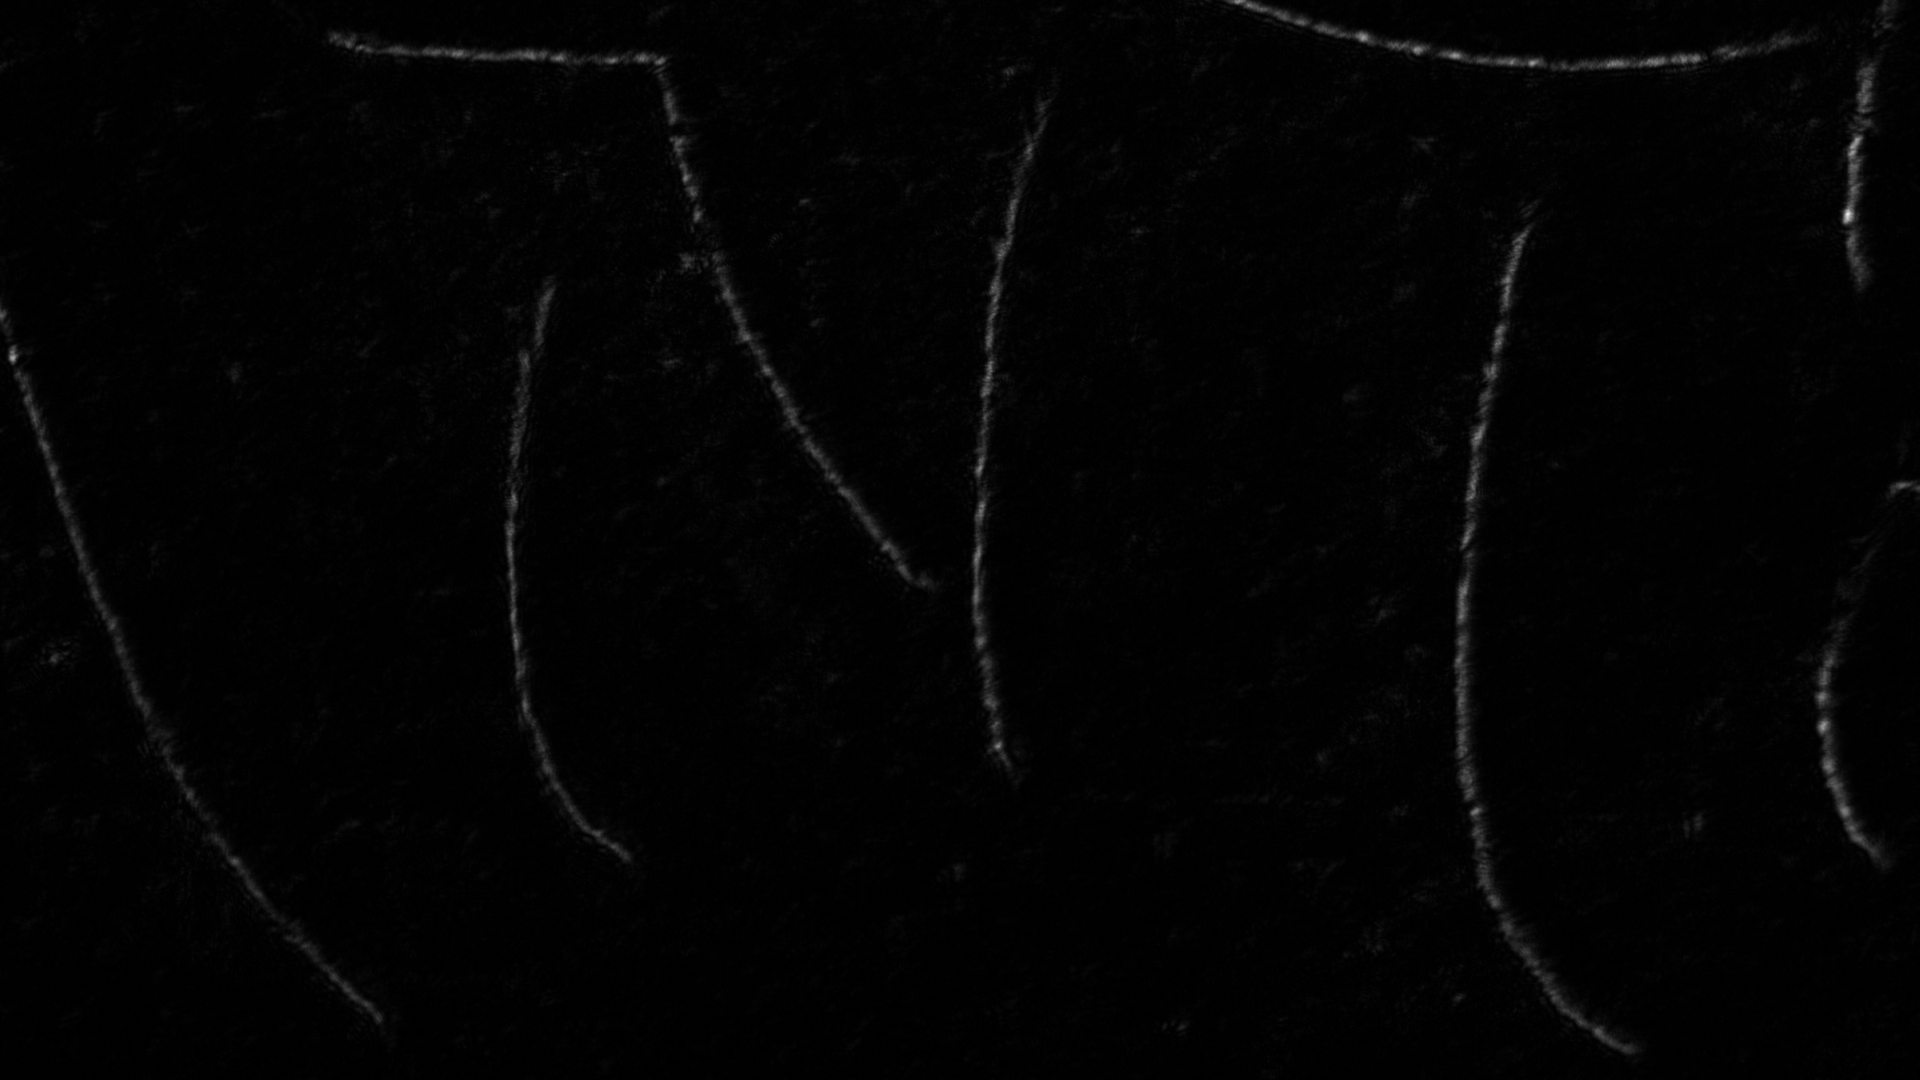
\includegraphics[width=\textwidth]{parte4-filtrado/4f-pic-2ocm-diafragm-10cm-camera-letters-high-frequency-dot-right-a-bit-down.png}
			\caption{Filtrado similar a \ref{fig:filtrado2}, pero en una dirección a un ángulo del eje vertical y horizontal}
		\end{subfigure}
		\caption{Realizando transformaciones con un diafragma en un sistema 4-f en medio del sistema, podemos realizar filtros de frecuencias analógicamente. Aquí podemos ver la imagen original (Fig.~\ref{fig:filtrado1}), y como podemos filtrar high-pass en distintas direcciones, obteniendo los bordes de las imágenes}
		\label{fig:filtrado:all}
	\end{center}
\end{figure}

\subsection{Cuestiones}
\subsubsection{¿Qué distancia focal tiene la lente más próxima a la camara? Justifique el procedimiento seguido para determinar el orden de las lentes.}
La distancia focal es de 10cm para esta práctica. Tenemos disponible otra lente de focal de 20cm, pero esto crearía una imagen mas grande, que preferimos sea la primera lente para tener un campo de Fourier más amplio.

\subsubsection{Elegir un filtro entre los estudiados en la práctica que podría ser adecuado para la observación de objetos semi-transparentes. Justifique la respuesta.}

A la hora de estudiar un objeto semi-transparente, lo que importe serán los bordes y características de detalle. Por lo tanto, usaremos un filtro pasa alta, para eliminar las frecuencias bajas de respuesta, que representan el campo medio


\subsubsection{¿Qué observamos en la salida del sistema si usamos como filtro una red periódica? Justifique la respuesta.}
Si utilizamos como filtro una red periódica, estamos multiplicando la transformada de Fourier con la red periódica. Y, por ello, en la respuesta obtendremos la convolución entre la imagen y la Fourier de la red periódica.

Como la Fourier de la red periódica será representada por unos desplazamientos, obtendremos como el resultado la misma imagen múltiples veces. Estos resultados se pueden ver en \ref{fig:filtrado:all}

\begin{figure}[hptb]
	\begin{center}
		\begin{subfigure}[t]{0.3\textwidth}\centering
			
\includegraphics[width=\textwidth]{talbot-4f/letters-guion-nothing-in-middle}
			\caption{Imagen sin el filtro}
			\label{fig:filtrado:talbot:1}
		\end{subfigure}
		\quad
		\begin{subfigure}[t]{0.3\textwidth}\centering
			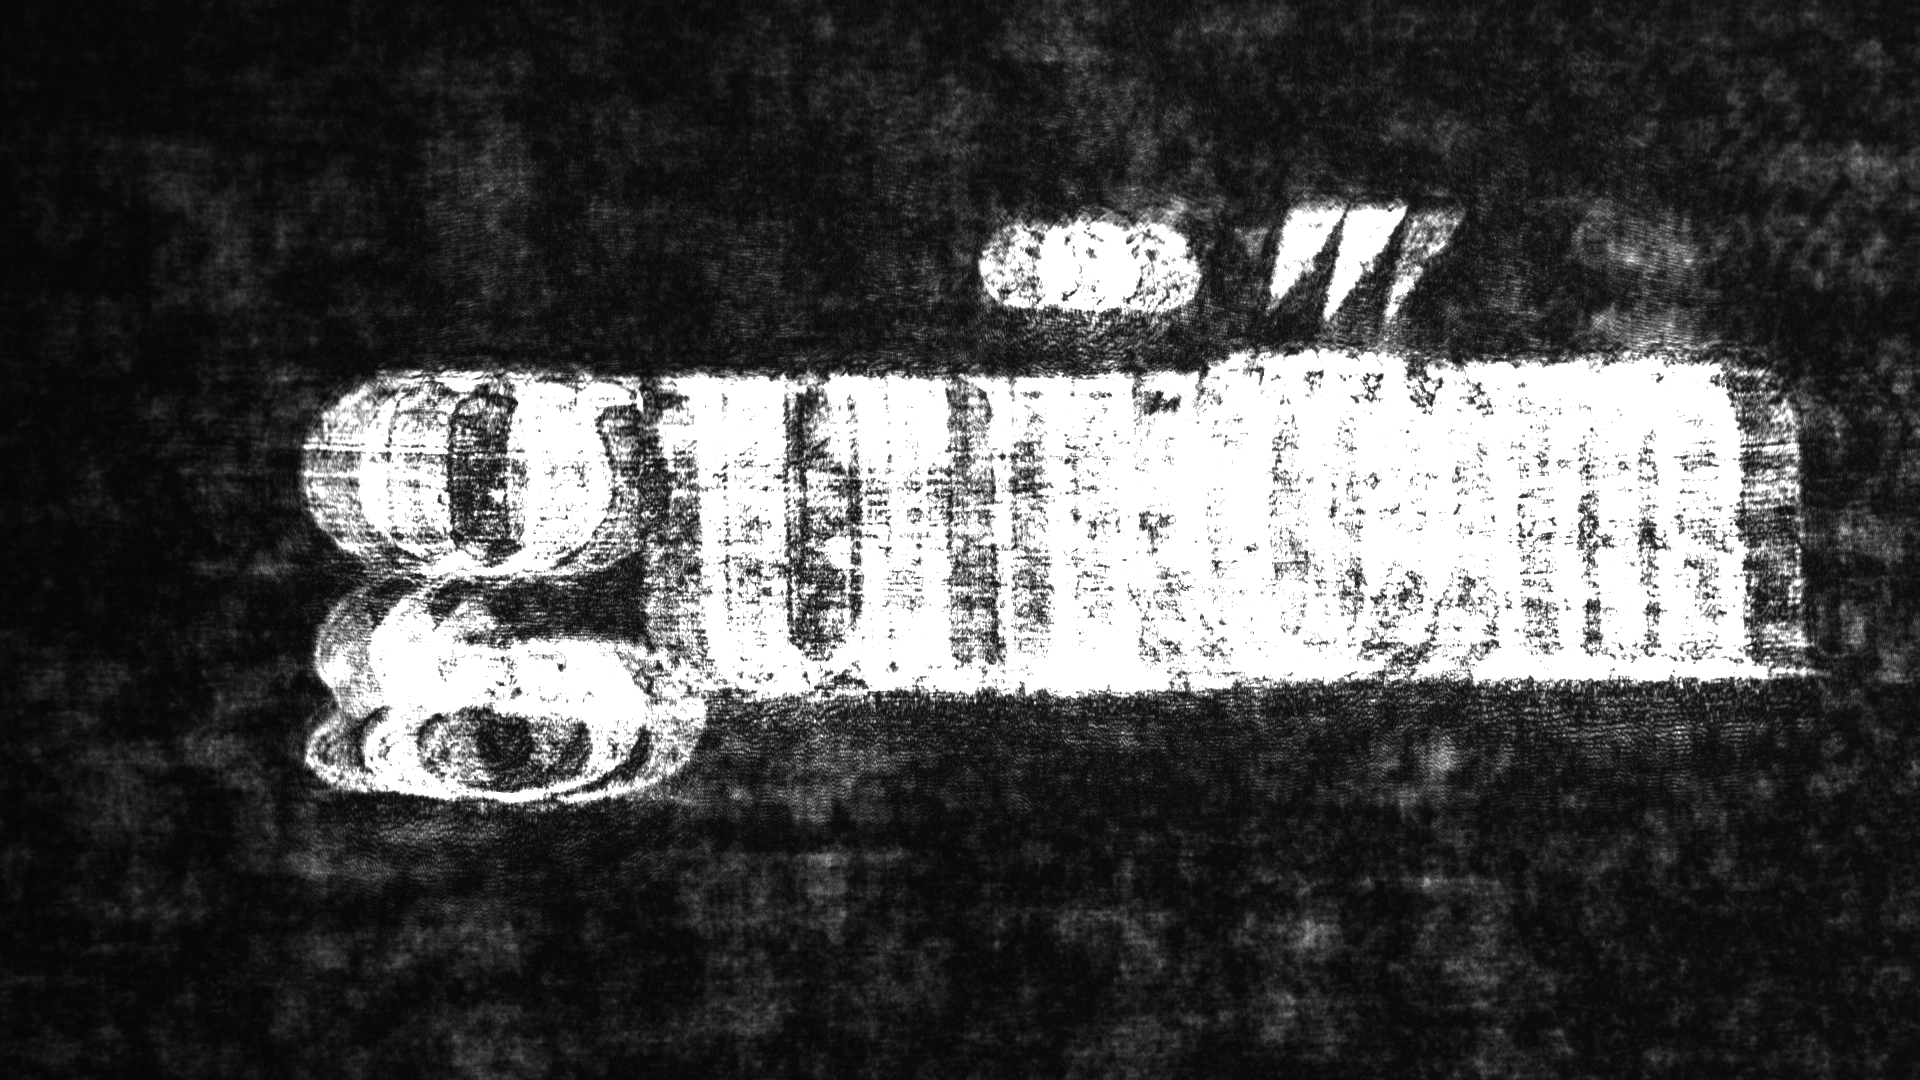
\includegraphics[width=\textwidth]{talbot-4f/letters-guion-horizontal-grading}
			\caption{Imagen con un filtro periódica horizontal}
			\label{fig:filtrado:talbot:2}
		\end{subfigure}
		\quad
		\begin{subfigure}[t]{0.3\textwidth}\centering
			
\includegraphics[width=\textwidth]{talbot-4f/letters-guion-vertical-grading}
			\caption{Imagen con la red periódica vertical}
			\label{fig:filtrado:talbot:3}
		\end{subfigure}
		\caption{Realizando un filtro en un sistema 4-f usando una red periódica en el campo de Fourier del sistema 4-f. Se observa como esto produce la convolución de la imágen con el sistema, creando una imagen periódica}
		\label{fig:filtrado:all}
	\end{center}
\end{figure}


\section{Formación de imágenes con luz parcialmente coherente}

En esta sección comparamos los efectos de iluminar el objeto con luz coherente y con luz incoherente. Para generar la iluminación incoherente se utilizó un difusor girando. En la figura ~\ref{fig:coherente} y ~\ref{fig:incoherente} se muestran los efectos de iluminar con sendos tipos de fuente.

\subsection{Cuestiones}
\subsubsection{¿El rango de distancias donde observamos la imagen del objeto 2D es mayor en el caso iluminación coherente o parcialmente coherente? ¿Qué iluminación es mejor para la observación de objetos 3D?}

Con luz coherente podemos observar objetos en muchos planos distintos a la vez, sin embargo, con luz incoherente, solo los podemos observar cuando estén en un plano que formen imagen en nuestro receptor, en cualquier otro plano crearán una imagen difusa.

Para la observación de objetos 3D la iluminación coherente es mejor, si podemos usar técnicas en las que separemos la fase y filtremos la imagen adecuadamente para extraer más información. Si lo que queremos es obtener un plano del objeto 3D, con luz incoherente, enfocaremos solo en ese plano.

\begin{figure}[h]
    \centering
    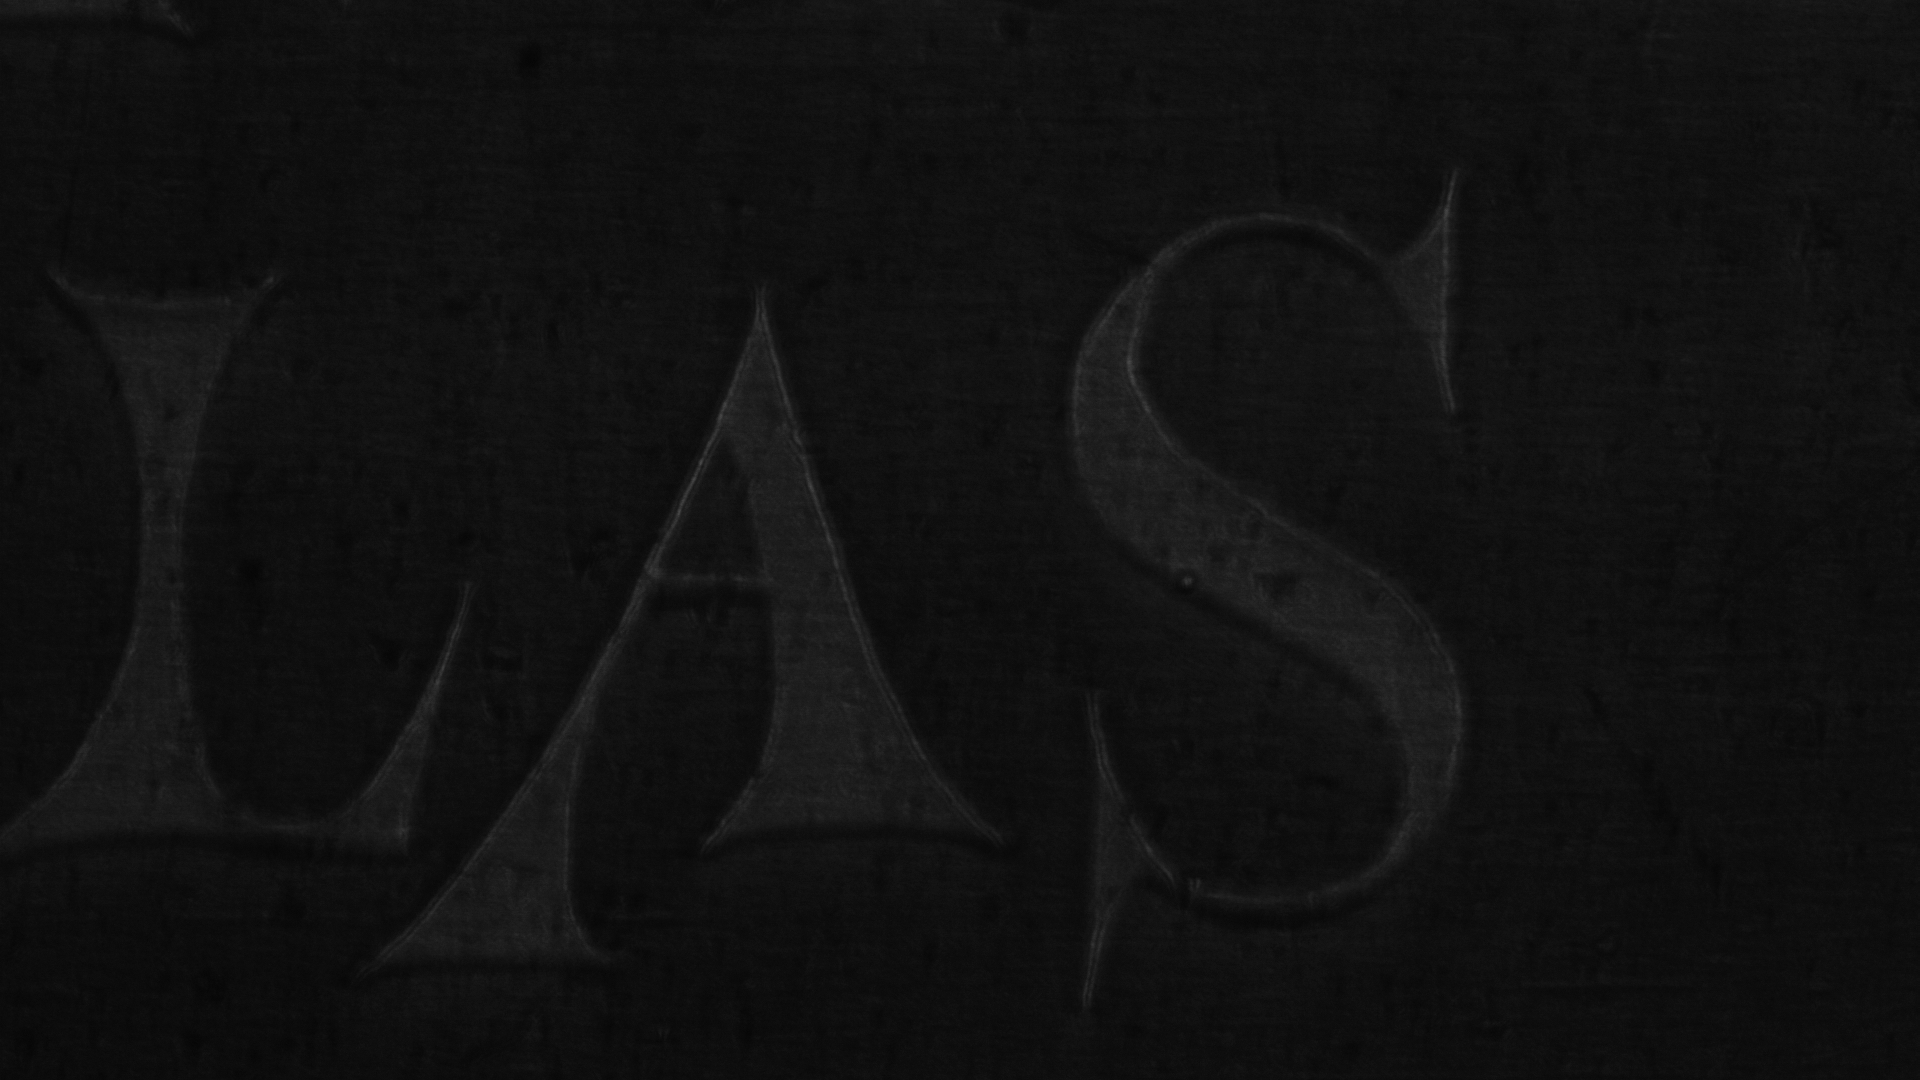
\includegraphics[scale=0.18]{parte5-luz-coherente/imagen-letras-con-difusor-y-grating.png}
    \caption{Imagen con iluminación incoherente}
    \label{fig:incoherente}
\end{figure}

\begin{figure}[h]
    \centering
    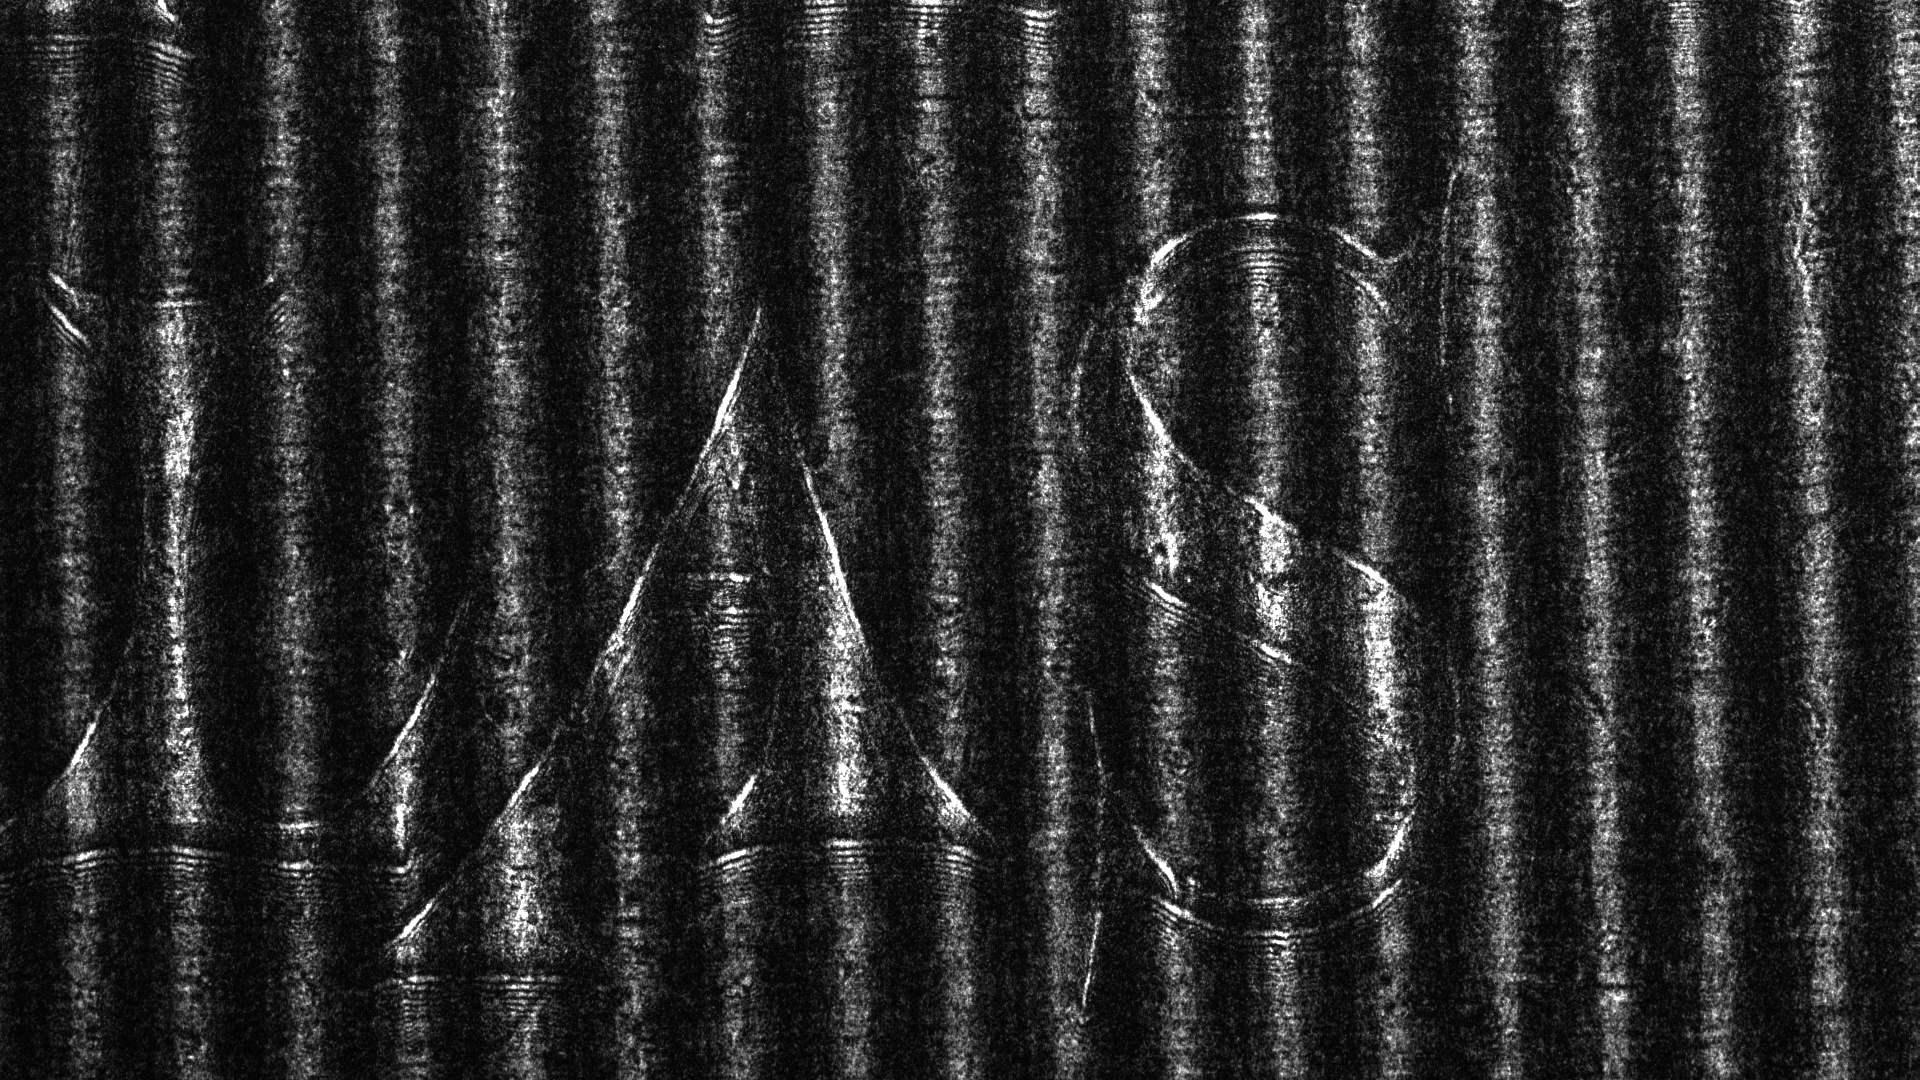
\includegraphics[scale=0.18]{parte5-luz-coherente/imagen-letras-no-difusor-y-grating.png}
    \caption{Imagen con iluminación coherente}
    \label{fig:coherente}
\end{figure}

%%%%%%%%%% If using BibTeX:
%\bibliography{bibliography}

\end{document}
